% Encoding:UTF-8
% Copyright 2014 MathFire
% Author: Rickjin (ZhihuiJin@gmail.com)
%
\chapter{神奇的伽玛函数}

\section{开篇}

数学爱好者们汇集在网络论坛上的一大乐事就是对各类和数学相关的事物评头论足、论资
排辈。如果要评选历史上最伟大的数学家,就会有一大堆的粉丝围绕高斯、黎曼、牛顿、
欧拉、阿基米德等一流人物展开口水战;如果要讨论最奇妙的数学常数,$e, \pi,
\phi=\frac{\sqrt{5}-1}{2} $ 肯定在候选队列中;如果要推举最美丽的数学公式,欧拉
公式 $e^{i\pi} + 1= 0$  与和式 $ 1 + \frac{1}{2^2} + \frac{1}{3^2} +
\frac{1}{4^2} +  \cdots  = \frac{\pi^2}{6} $ 常常被数学爱好者们提及;如果有人追
问最神奇的数学函数是什么? 这个问题自然又会变得极具争议,而我相信如下这个长相有
点奇特的伽玛函数
$$ \Gamma(x)=\int_0^{\infty}t^{x-1}e^{-t}dt $$
一定会出现在候选队列中。 

伽玛函数不是初等函数,而是用积分形式定义的超越函数,怎么看都让人觉得不如初等函
数自然亲切。然而伽玛函数也被称为阶乘函数,高等数学会告诉我们一个基本结论:伽玛函
数是阶乘的推广。通过分部积分的方法,容易证明这个函数具有如下的递归性质
$$\Gamma(x+1) = x \Gamma(x)$$
由此可以推导出,对于任意的自然数$n$
$$\Gamma(n) = (n-1)! .$$
由于伽玛函数在整个实数轴上都有定义,于是可以看做阶乘概念在实数集上的延拓。

如果我们继续再学习一些数学,就会惊奇地发现这个具有神秘气质的伽玛函数真是才华横
溢。她栖身于现代数学的各个分支,在微积分、概率论、偏微分方程、组合数学, 甚至是
看起来八竿子打不着的数论当中,都起着重要的作用。 并且这个函数绝非数学家们凭空臆
想的一个抽象玩具,它具有极高的实用价值,频繁现身于在现代科学尤其是物理学之中。

笔者对数学的涉猎很有限,主要是从概率统计中频繁地接触和学习这个函数,不过这个函数
多年来一直都让笔者心存疑惑:
\begin{enumerate}
\item 都说$n!$ 和伽玛函数是近亲,可是从相貌上这两个数学公式都差了十万八千里,历
史上数学家们是如何找到这个奇特的函数的?
\item 现代数学对伽玛函数的定义使它满足 $\Gamma(n) = (n-1)!$,既然号称是$n!$ 的推广,
为何定义伽玛函数的时候不让它满足$\Gamma(n) = n!$?这看起来不是更加舒服自然吗?
\item 伽玛函数是唯一满足阶乘特性的推广函数吗?
\item 伽玛函数在各种概率分布的密度函数中频繁出现,伽玛函数本身是否有直观的概率
解释?
\end{enumerate}

带着这些疑问,笔者翻阅了许多讲解伽玛函数历史和应用的资料,发现伽玛函数真是一个
来自异族的美女,与生俱来携带着一种神秘的色彩。你要接近她并不难,然而她魅力独特
,令你无法看透。从她出生开始,就吸引着众多一流的数学家对她进行解读。 历史上伽
玛函数的发现,和数学家们对阶乘、插值以及积分的研究有着紧密的关系,而这最早要从
著名的沃利斯公式讲起。

\section{无心插柳 --- 沃利斯公式}

1655年, 英国数学家沃利斯(John Wallis, 1616-1703)写下了一个神奇的数学公式
\begin{equation}
\label{wallis-formula}
\frac{2}{1} \cdot \frac{2}{3} \cdot \frac{4}{3} \cdot \frac{4}{5} \cdot
\frac{6}{5} \cdot \frac{6}{7} \cdot \frac{8}{7} \cdot \frac{8}{9} \cdot \cdots =
\frac{\pi}{2} .
\end{equation}
$\pi$ 居然可以如此齐整地表示成奇数、偶数的比值,着实令人惊讶。 历史上数学家们为
了寻求对$\pi$ 这个迷人的常数更加深刻的理解,前赴后继倾注了无数的精力。数学家们
发现,$\pi$ 可以表达成许许多多奇妙的形式,而沃利斯公式是欧洲历史上发现的第二
个把 $\pi$ 表达成式了无穷序列的形式, 由于它简洁的对称美,也成为了许多数学人经
常提及的数学公式之一。为何沃利斯公式会和伽玛函数发生联系呢?实际上对沃利斯公式
做一下变形整理就可以得到如下等价形式
$$ \lim_{n\rightarrow\infty} \frac{(2^n \cdot n!)^4}{[(2n)!]^2(2n+1)} = \frac{\pi}{2} $$
我们看到了阶乘,所以沃利斯公式天然和阶乘有着紧密的联系。

\begin{figure}[htbp]
\centering
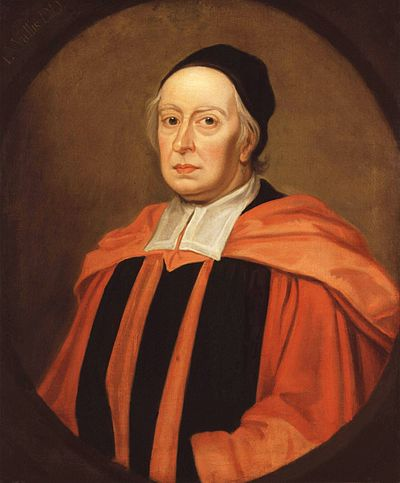
\includegraphics[width=0.25\textwidth]{gamma/john-wallis.jpg}
\caption{沃利斯}
\end{figure}

我们先来欣赏一下沃利斯公式的证明。利用现代数学分析的知识证明这个公式并不难,通
常微积分课本对这个公式的证明是从积分式
$$ I(n) = \int_0^\pi \sin^nxdx $$
出发,通过分部积分得到一个关于$I(n)$ 的递推公式,反复使用这个递推公式就可以证明
结论。 不过这个证明思路有点繁琐,数学家波利亚(George P\'{o}lya, 1887-1985) 在它
的名著《数学与猜想》中提到了另外一个非常简洁、符合直觉,但是不够严格的证明
思路,其中用到的最重要的公式是数学家欧拉(Leonhard Euler, 1707-1783)提供的。欧拉
当年研究正弦函数 $\sin x$ 的时候,发现该函数有无穷多个零点 $0, \pm\pi, \pm
2\pi, \pm 3\pi, \cdots $。 而一个多项式$f(x)$ 如果有零点 $x_1, x_2, \cdots,
x_n$(此处$x_i, x_j$ 可以相同, 对应于有重根的情形), 那么 $f(x)$ 一定可以表示为 
$$ f(x) = a_0 (x-x_1) (x-x_2) \cdots (x-x_n) .$$ 
于是欧拉大胆地猜测 $\sin x$ 也具有多项式的这种性质,即
\begin{equation}
\label{euler-sinx}
\sin x = x \prod_{n=1}^\infty\left(1 - \frac{x^2}{n^2\pi^2}\right) 
= x (1- \frac{x^2}{\pi^2})  (1- \frac{x^2}{4\pi^2})  (1- \frac{x^2}{9\pi^2}) \cdots .
\end{equation}
理工科背景的学生大都学习过 $\sin x$ 的泰勒展开式, 通常只有数学背景的学生才会接
触到这个 $\sin x$ 的无穷乘积展开式。这个展开式在数学推导中有许多妙用。数学史
上它发挥的第一个重要作用,就是帮助欧拉推导出了如下美丽的公式
$$ 1 + \frac{1}{2^2} + \frac{1}{3^2} + \frac{1}{4^2} +  \cdots  = \frac{\pi^2}{6} . $$ 
这个展开式子的另一个妙处就是可以用于证明沃利斯公式, 不过这个思路并非欧拉本人给
出,而是后来的数学家发现的。 在\eqref{euler-sinx} 式中取 $x=\frac{\pi}{2}$, 可
以得到
$$ 1 = \frac{\pi}{2} \prod_{n=1}^\infty\left(1 - \frac{1}{4n^2}\right)
= \frac{\pi}{2} \prod_{n=1}^\infty\left(\frac{2n-1}{2n} \cdot \frac{2n+1}{2n}\right) 
$$
所以
$$ \frac{\pi}{2} = \prod_{n=1}^\infty\left(\frac{2n}{2n-1} \cdot \frac{2n}{2n+1}\right) 
$$
上式就是沃利斯公式。之所以说以上的证明思路不够严格,是由于欧拉给的$\sin x$ 无穷
乘积展开式的严格证明并不简单,依赖于现代数学分析理论。 

欣赏完沃利斯公式的证明,我们把镜头重新拉回到沃利斯生活的年代,要知道沃利斯给出
这个公式是在 1655 年,那时候牛顿刚满13岁,莱布尼茨更小,欧拉还没出生,整个欧洲
数学界对微积分的认识还停留在非常粗糙的阶段,对正弦函数 $\sin x$ 的认识也非常有
限, 所以沃利斯当然不可能用上述的思路找到他的公式, 那沃利斯是如何发现这个
$\pi$ 的无穷乘积表达式的呢?

在沃利斯的时代,微积分有了初步的进展,当时考虑的典型的问题就是求一个曲线和坐标
轴围成的面积。欧洲的数学家们追寻阿基米德一千多年前开创的穷竭法,把曲线下的面积
表达为求无穷多个矩形面积的和。当积分的思想在十七世纪开始逐步发酵的时候,沃利斯
已经能够运用积分的思路处理一些简单曲线的面积。譬如,对于最简单的幂函数曲线
$y=x^n$,使用我们现在的数学记号, 沃利斯时代的数学家们获得了如下的结果
$$ \int_0^1 x^n dx = \frac{1}{n+1},  n=0,1,2,\ldots .$$

\begin{figure}[htbp]
\centering
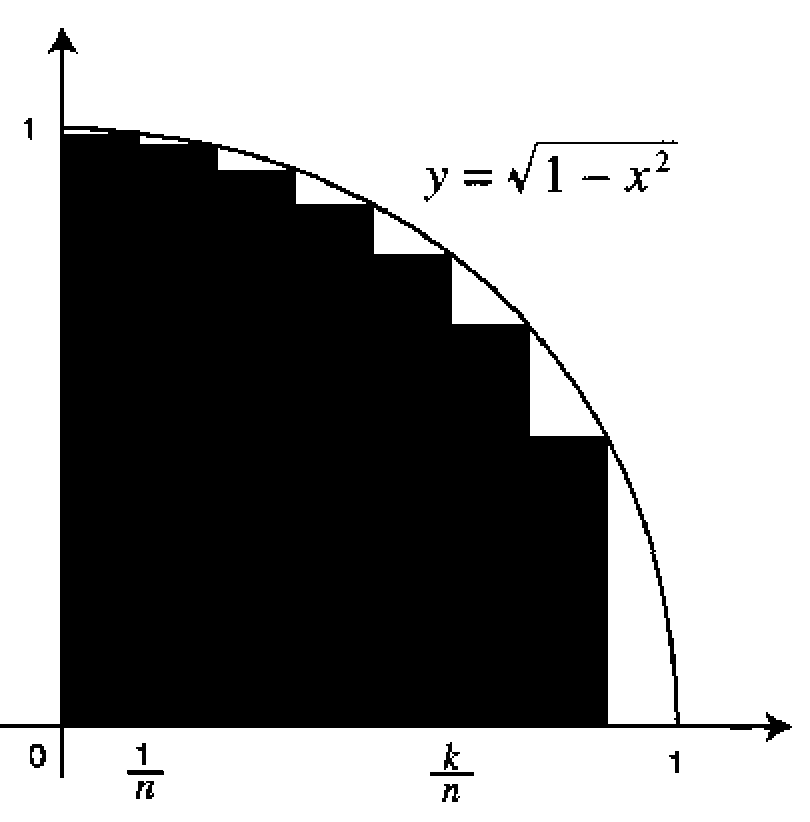
\includegraphics[width=0.5\textwidth]{gamma/circle-area.png}
\caption{求圆弧下的面积}
\end{figure}

圆的面积一直是千百年来数学家们深入关心和研究的问题,很自然地沃利斯也想到了可以
使用同样的思路来处理圆的面积。 不过数学家们早已经证明道圆的面积是 $\pi r^2$,用
积分的方法去计算圆的面积能带来什么好处呢? 沃利斯在此做了一个逆向思维,他的真实
目标并不是要计算圆的面积,而是冲着$\pi$ 去的。 沃利斯的一个漂亮的思路是:我们已
经知道四分之一的单位圆圆弧 $y=\sqrt{1-x^2} (0 \le x \le 1)$ 和坐标轴围成的面积
是 $\frac{\pi}{4}$, 如果这个面积能通过无穷分割的方法表达成一个解析表达式,那我
们其实就可以得到计算 $\pi$ 的一个解析表达式。

然而沃利斯在处理这个圆弧下的面积的时候遇到了困难。虽然基于无穷分割的方法可以得到 
$$ \int_0^1 (1-x^2)^{1/2} dx = \lim_{n\rightarrow \infty} \frac{1}{n} \sum^n_{k=1} \sqrt{1-\frac{k^2}{n^2}}$$ 
但是这个极限难以简化计算。 沃利斯天才的地方就是换了一个更一般的思路来处理这个问题:
\begin{enumerate}
\item 考虑更一般的曲线面积问题
$$ A_{p,q} = \int_0^1 (1-x^\frac{1}{p})^q dx$$ 
原来的问题变成了一个特例,就是计算 $A_{\frac{1}{2},\frac{1}{2}}$ ;

\item 对$p,q$ 为整数的情况做计算,并系统地列成表格, 从表格中观察变化规律,总结出一般的公式;
\item 把计算公式从$p,q$为整数的情形延拓、内插到分数的情形,从而计算出
$A_{\frac{1}{2},\frac{1}{2}}$ 。
\end{enumerate}

沃利斯对 $p,q = 1,2,\ldots,10$ 做了计算, 发现$A_{p,q}$ 这个表格不太好看,改为
倒数之后容易分析。于是取 $B_{p,q} = \frac{1}{A_{p,q}}$, 列出表格一看, 居然恰好
是帕斯卡三角形! 这个三角形中的组合数已经是数学家们熟悉知的, 于是沃利斯很容易
地得到
\begin{equation}
\label{wallis-Bpq}
B_{p,q} = \frac{(p+q)!} {p! q!} = \frac{1}{p!} (q+1) (q+2) \ldots (q+p), q=0,1,2 \ldots
\end{equation}
由上式进一步可以得到如下的递推公式
\begin{equation}
\label{wallis-Bpq-recursion}
B_{p,q} = \frac{p+q}{q} B_{p,q-1}
\end{equation}
原始的问题就转化为计算 $B_{\frac{1}{2},\frac{1}{2}}$。 由此开始, 沃利斯开始了
他天才的推广:
\begin{enumerate}
\item 虽然 \eqref{wallis-Bpq} 和 \eqref{wallis-Bpq-recursion}是基于$p,q$ 为整数得到
的, 但是沃利斯认为这个公式也应该适用于分数的情形;
\item 由于原始表格是对称的, 沃利斯相信推广到分数之后的表格依然保持对称性。
\end{enumerate}

\begin{table}[htb]
\centering
\caption{$B_{pq}$ 数值表}
\begin{tabular*}{0.8\textwidth}{@{\extracolsep{\fill}}|c|ccccccc|}
\hline
\diagbox{p}{q} & 0 & 1 & 2 & 3 & 4 & \ldots & 10 \\
\hline
0 & 1 & 1 & 1 & 1 & 1 & \ldots & 1  \\
1 & 1 & 2 & 3 & 4 & 5 & \ldots & 11  \\
2 & 1 & 3 & 6 & 10 & 15 & \ldots & 66  \\
3 & 1 & 4 & 10 & 20 & 35 & \ldots & 286  \\
4 & 1 & 5 & 15 & 35 & 70 & \ldots & 1001  \\
\vdots & \vdots & \vdots & \vdots & \vdots & \vdots & \vdots & \vdots  \\
10 & 1 & 11 & 66 & 286 & 1001 & \ldots & 184756  \\
\hline
\end{tabular*}
\end{table}

基于对称性假设和计算式\eqref{wallis-Bpq}, 我们可以得到,
$$ B_{\frac{1}{2}, 1} =  B_{1, \frac{1}{2}} = \frac{1}{1!}(\frac{1}{2} + 1)  =  \frac{3}{2} $$
考虑 $p=\frac{1}{2}$ 的情形, 重复使用迭代公式 \eqref{wallis-Bpq}, 容易得到
$$ B_{\frac{1}{2}, m} = \frac{2m+1}{2m}\cdot \frac{2m-1}{2m-2} \ldots \frac{5}{4} \cdot\frac{3}{2} $$
$$ B_{\frac{1}{2}, m+\frac{1}{2}} = \frac{2m+2}{2m+1} \cdot\frac{2m}{2m-1} \ldots \frac{4}{3} 
\cdot B_{\frac{1}{2}, \frac{1}{2}} $$
由于 $B_{\frac{1}{2}, q}$  是基于$q$ 递增的,所以有
$$ B_{\frac{1}{2}, m-\frac{1}{2}} < B_{\frac{1}{2}, m}  < B_{\frac{1}{2}, m+\frac{1}{2}}  $$
利用\eqref{wallis-Bpq-recursion} 式这个递推公式,马上可以得出上式两端有相同的极限
$$ \lim_{m \rightarrow \infty} B_{\frac{1}{2}, m+\frac{1}{2}} 
= \lim_{m \rightarrow \infty} \frac{2m+2}{2m+1}  B_{\frac{1}{2}, m-\frac{1}{2}} 
= \lim_{m \rightarrow \infty} B_{\frac{1}{2}, m-\frac{1}{2}} .
$$  
于是,利用两侧极限的夹逼,可以得到
$$ \lim_{m \rightarrow \infty} B_{\frac{1}{2}, m} = \lim_{m \rightarrow \infty} B_{\frac{1}{2}, m+\frac{1}{2}}  $$
即有
$$ 
\frac{3}{2} \cdot \frac{5}{4} \cdot \cdots \cdot \frac{2m-1}{2m-2} \cdot \frac{2m+1}{2m} \cdots 
= B_{\frac{1}{2}, \frac{1}{2}} \cdot \frac{4}{3} \cdot \cdots \cdot \frac{2m}{2m-1} \cdot  \frac{2m+2}{2m+1} \cdot \cdots
$$
所以
$$ 
\frac{2}{B_{\frac{1}{2}, \frac{1}{2}}} = \frac{2}{1} \cdot\frac{2}{3} \cdot\frac{4}{3}\cdot \frac{4}{5}\cdot
\cdots \cdot \frac{2m-2}{2m-1}\cdot \frac{2m}{2m-1} \cdot \frac{2m}{2m+1} \cdot \frac{2m+2}{2m+1} \cdot\cdots
$$
由于 $\displaystyle \frac{2}{B_{\frac{1}{2}, \frac{1}{2}}} = 2A_{\frac{1}{2}, \frac{1}{2}} = \frac{\pi}{2} $, 
代入上式就得到了沃利斯公式 \eqref{wallis-formula}。

上述推导的基本思想是在沃利斯的名著《无穷分析》(Arithmetica Infinitorum,1655)
中给出的。沃利斯公式对$\pi$ 的表示如此的奇特,以至于惠更斯第一次看见这个公式的
时候根本不相信,直到有人给惠更斯展示了利用该公式对$\pi$做近似计算,才消除了惠更
斯的疑惑。沃利斯是在牛顿之前英国最有影响力的数学家,他的这本书包含了现代微积分
的先驱工作,给后来的数学家包括牛顿、斯特林、欧拉都产生了重要的影响。牛顿1642年
在老家研读沃利斯的这本书的时候受到启发,从而把二项式定理从整数的情形推广到了分
数的情形,这也是牛顿有生以来的第一个数学发现;而牛顿后续在微积分上的工作也同样
受到了沃利斯的深刻影响。 

回过头来我们观察一下沃利斯公式推导过程中使用的\eqref{wallis-Bpq} 式,这个组合公
式中实际上包含了阶乘$p!$、 $q!$, 当沃利斯认为这个公式也适合于$p, q$ 为分数的情
形的时候,隐含了一个假设是阶乘这个源自整数的概念是可以推广到分数的情形的。虽然
沃利斯并没有显示地提出把阶乘推广到分数的问题, 沃利斯对一些特殊积分式的研究、沃
利斯公式的结论以及推导过程却给后来的数学家们进一步研究阶乘提供了许多重要的线索
,也为未来伽玛函数的发现埋下了一颗种子。 

\section{近似与插值的艺术}

十七世纪中期,由于帕斯卡、费马、贝努利等数学家的推动,概率论以及与之相关的组合
数学获得了很大的发展,阶乘的数值计算开始频繁的出现在数学家面前。 真正的开始对
$n!$ 进行细致地研究并取得突破的,是数学家棣莫弗(Abraham de Moivre, 1667-1754)和
斯特林(James Stirling, 1692-1770)。

\begin{figure}[htbp]
\centering
\vspace{1cm}
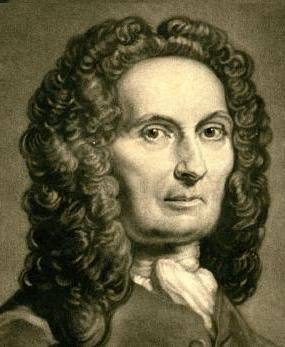
\includegraphics[width=0.2\textwidth]{gamma/abraham-de-moivre.jpg}
\caption{棣莫弗}
\end{figure}

棣莫弗从1721年开始考虑二项分布的概率计算问题,其中一个问题是:当$n \rightarrow
\infty $时,如何计算对称二项分布的中间项的概率
$$ b\left(n, {1\over2}, {n \over 2}\right) = \binom{n}{{n \over 2}} 
\left(\frac{1}{2}\right)^n 
= \frac{n!}{({n\over 2})! \cdot ({n \over 2})!} \left(\frac{1}{2}\right)^n .$$
上式中假设了$n$为偶数。棣莫弗经过一番复杂的推导计算,得到了如下的结果
$$ b\left(n, {1\over2}, {n\over2}\right) \approx  2.168 \frac{(1 - {1\over n})^n} {\sqrt{n-1}} 
\approx \frac{2.168 e^{-1}}{\sqrt{n}}.$$
1725年,斯特林得知了棣莫弗的研究问题和结果,这激起了他浓厚的兴趣。斯特林经过更
细致的推导,得到了如下更加漂亮的结果
$$ b\left(n, {1\over2}, {n\over2}\right) \approx \sqrt{\frac{2}{\pi n}} .$$
斯特林写信告知了棣莫弗他的推导结果,斯特林的结果中最引人注目的地方就是 $\pi$ 的
引入,这给棣莫弗很大的启发。 基于上述二项概率计算的研究,棣莫弗最终给出了如下重
要公式
$$ n! \approx C \sqrt{n} \left(\frac{n}{e}\right)^{n} $$
$C$ 是一个常数。而在斯特林推导$b(n, {1\over2}, {n\over2})$ 过程中引入 $\pi$ 的
启发下, 1730 年棣莫弗利用沃利斯公式推导出了 $C = \sqrt{2\pi}$,也就是得到了斯
特林公式
$$ n! \approx \sqrt{2\pi n} \left(\frac{n}{e}\right)^{n} .$$
所以现代数学史的研究大都认为斯特林公式的最主要贡献者是棣莫弗,斯特林的贡献主要
在常数$C$ 的确定。 不过科学发展史中长期以来都存在一个被称之为 Stigler's Law 的
著名现象:绝大多数科学成果的冠名,大都不是历史上首位发现者的名字。或许这主要是
由于早年通信不发达、信息传播成本太高导致的。如今互联网如此的发达,学术界任何重
要的科研进展都可以快速传导到世界各地,这种问题发生的概率大大的降低了,类似牛顿
、莱布尼茨这种微积分发明权的世纪争夺战不太可能在这个时代重现。 

斯特林公式自发现以来,就吸引众多的数学家对它进行研究,提出了多种多样的证明方法
。实际上,从沃利斯公式出发就可以证明斯特林公式,甚至可以进一步证明斯特林公式和
沃利斯公式是完全等价的。在多种证明方法中,有一个基于概率论的证明思路:利用泊
松分布的特性,再加上中心极限定理,我们可以简洁地推导出斯特林公式。

假设 $X_1, X_2,\ldots, X_n $独立同分布, 都是服从参数 $\lambda=1$ 的泊松分布的
随机变量,取 $S_n=\sum_{i=1}^n X_i$, 则由泊松分布的可叠加性, 容易知道 $S_n
\sim Poisson(n)$, 于是由泊松分布的性质可知$S_n$ 的均值和方差都是 $n$, 利用中心
极限定理可以得到
$$ Z_n = \frac{S_n - E(S_n)}{\sqrt{ Var(S_n) }} = \frac{S_n - n}{{\sqrt n }} 
\rightarrow Z, \quad Z \sim N(0,1) $$
$Z$ 为正态分布随机变量,密度函数为
$$ \displaystyle f(z)=\frac{1}{\sqrt{2\pi}}e^{-\frac{z^2}{2}} .$$
所以,我们有如下推导
\begin{eqnarray*}
\begin{array}{lll}
P\{{S_n} = n\} & = & \displaystyle P\{ n - 1 < {S_n} \le n\}  \\ 
              & = & \displaystyle P\{ -\frac{1}{{\sqrt n }} < \frac{{{S_n} - n}}{{\sqrt n }} \le 0\}  \\ 
              & \approx  & \displaystyle P\{ -\frac{1}{{\sqrt n }} < Z \le 0\}  \\ 
 & = & \displaystyle \int_{ - \frac{1}{{\sqrt n }}}^0 f(z) dz  \\ 
 & \approx & f(0) [0 - ( - \frac{1}{{\sqrt n }})] \\
 & = & \displaystyle \frac{1}{\sqrt{2\pi n}} .\\
\end{array}
\end{eqnarray*}
由于$S_n$ 符合参数$\lambda =n$ 的泊松分布,实际上有
$$ P\{ {S_n} = n\}  = \frac{{{e^{ - n}}{n^n}}}{{n!}} .$$
综合以上推导可以得到
$$ \frac{{{e^{ - n}}{n^n}}}{{n!}} \approx \frac{1}{\sqrt{2\pi n}}. $$
上式稍微整理一下就得到斯特林公式。这个推导的思路看起来非常初等,但是由于中心极
限定理的严格证明非常困难,所以不能被认为是一个严格的初等证明。不过该推导让我们
从概率角度来理解斯特林公式,同时也解释了斯特林公式中的$\pi$ ,是由于正态分布的
引入导致的。

斯特林公式非常有用,通过它可以得出$n!$ 非常精确的估计值。虽然$n$ 足够大时绝对误
差可以超过任何数,但是相对误差却很小,并且下降得非常快,甚至当 $n$ 很小的时候,
斯特林公式的逼近都相当精确。
\begin{table}[htb]
\centering
\caption{斯特林公式计算精度}
\begin{tabular*}{0.9\textwidth}{@{\extracolsep{\fill}}|c|ccccc|}
\hline
$n$ & 1 & 2 & 5 & 10 & 100 \\
\hline
$n!$ & 1 & 2 & 120 & 3628800 &  $\cdots$ \\
\hline
斯特林公式 & 0.9221 & 1.919 & 118.019 & 3598600 & $\cdots$ \\
\hline
相对误差 & 8\% & 4\% & 2\% & 0.8\%  & 0.08\% \\
\hline
\end{tabular*}
\end{table}

不过,斯特林对于 $n!$ 的研究实际上走得更远,而不是仅限于近似计算。追寻沃利斯和
牛顿在插值方面的工作,斯特林一直研究各种数列的插值问题,通俗地说就是把数列的通
项公式定义从整数集合延拓到实数集合。例如数列 $1,4,9,16,\cdots$ 可以用通项公式
$n^2$ 自然的表达,即便 $n$ 为实数,这个通项公式也是良定义的。直观地说就是可以找
到一条通过所有整数点$(n,n^2)$的平滑曲线$y=x^2$,从而可以把定义在整数集上的公
式延拓到实数集合。再比如求和序列 $1, 1+2, 1+2+3, 1+2+3+4, 1+2+3+4+5 \cdots$, 其
通项公式可以写为 $n(n+1)/2$ ,这个公式也可以很容易地延拓到实数集合上。 斯特林很
擅长于处理各种序列的插值问题,他在1730 年出版的一本书中描述了很多基于多阶差
分处理序列插值的方法,这些方法主要源自牛顿。 斯特林处理插值的思路稍微有点复杂,
我们不在此赘述,他的方法本质上类似于使用多项式曲线做插值。我们知道平面上两个
点可以确定一条直线,三个点可以确定一条抛物线,...,$n$+1 个点可以确定一条$n$次
多项式曲线。所以对于一个整数序列,如果我们无法直观地写出通项公式,为了计算某一
个实数点对应的值,可以用该实数点周围的 $n+1$个整数点去确定一条 $n$ 次多项式曲线
,从而可以基于拟合得到的多项式近似地计算实数点的值。

自然数的加法序列我们已经看到很容易做插值计算,对数学家们而言很自然的一个问题就
是:自然数的乘法序列 $1,1\cdot2, 1\cdot2\cdot3, 1\cdot2\cdot3\cdot4,
1\cdot2\cdot3\cdot4\cdot5,  \cdots$ 能否做插值计算?我们可以计算 $2!,3!$, 如何
计算 $(\frac{1}{2})!$呢?斯特林在他的书中开始考虑阶乘序列$1!, 2!,3!,4!,5!
\cdots$ 的插值问题。 如果我们把$(n,n!)$ 最初的一些点画在坐标轴上,确实可以看到
,容易画出一条通过这些点的平滑曲线。

\begin{table}[htb]
\centering
\begin{tabular*}{0.9\textwidth}{@{\extracolsep{\fill}}|cccccccccc|}
\hline
&&&&& n!的值 &&&& \\
$n$ & 1 & 2 & 3 & 4 & 5 & 6 & 7 & 8 & $\cdots$ \\
$n!$ & 1 & 2 & 6 & 24 & 120 & 720 & 5040 & 40320 & $\cdots$ \\
\hline
\end{tabular*}
\end{table}


\begin{figure}[htbp]
\centering
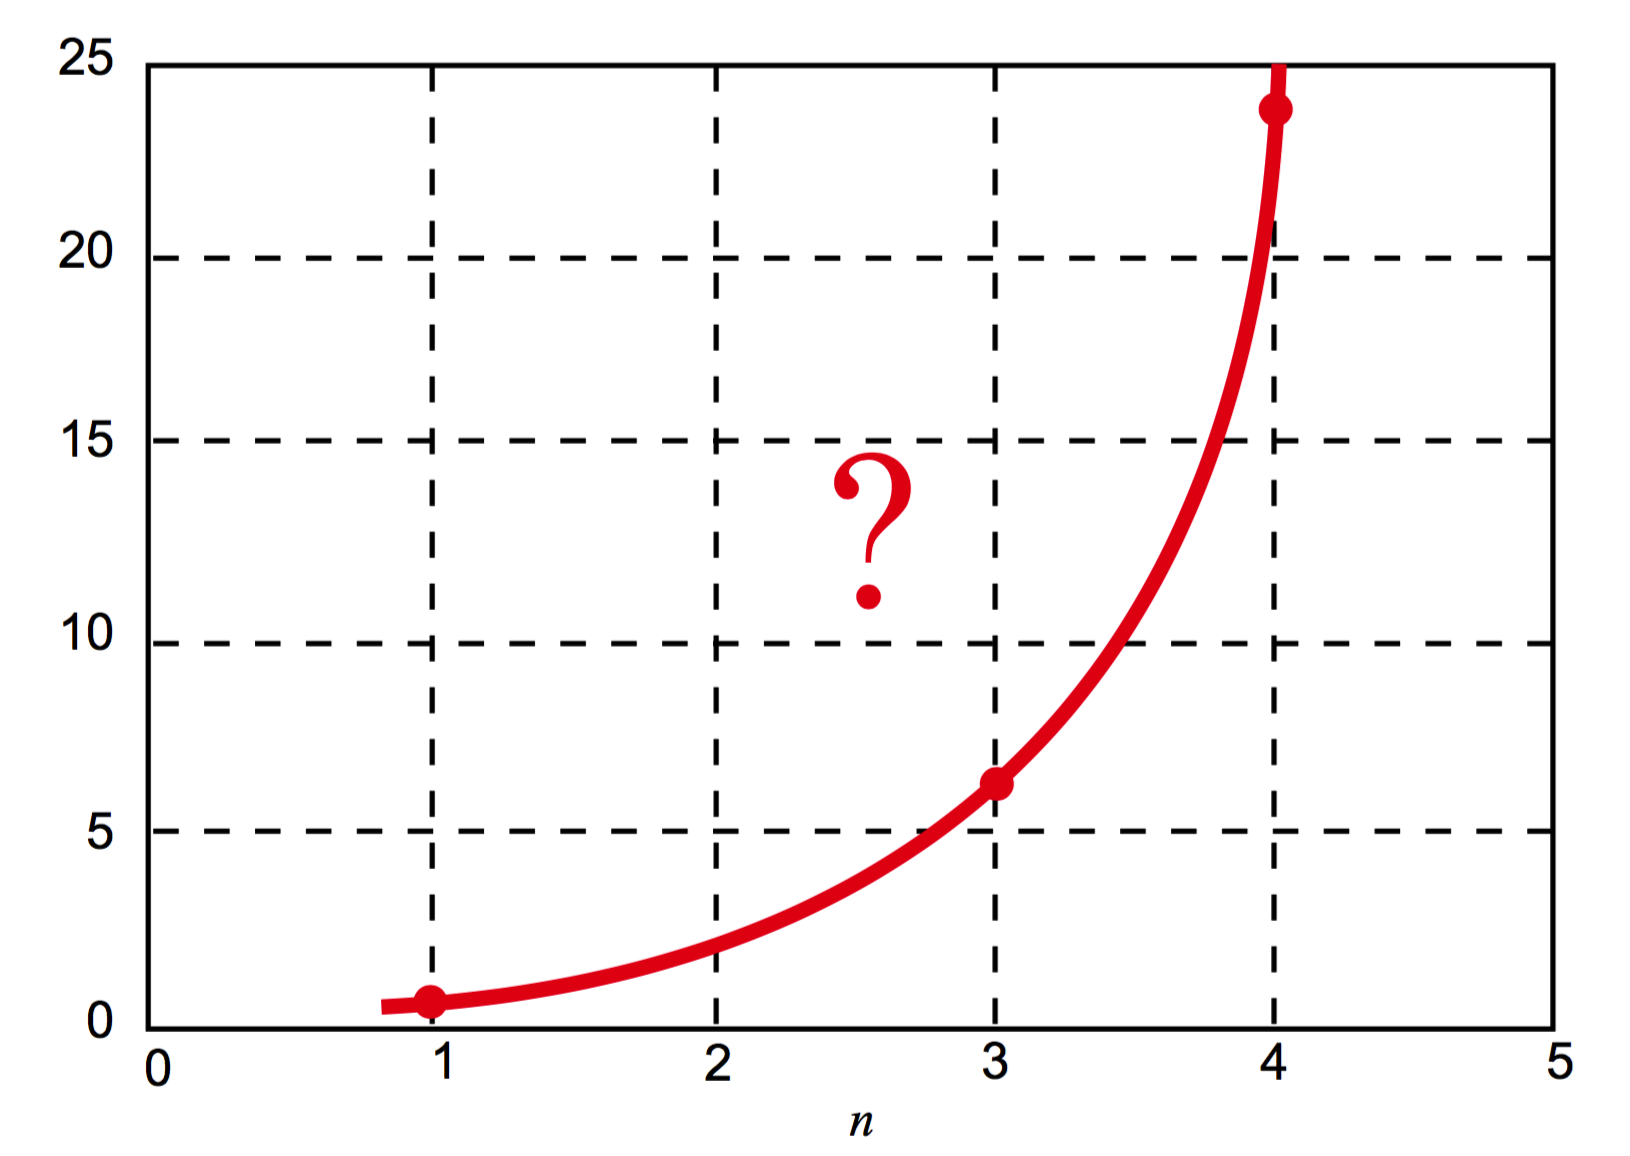
\includegraphics[width=0.6\textwidth]{lda/factorial-curve.png}
\caption{通过$(n,n!)$的曲线(替换该图片)}
\end{figure}

但是$n!$这个数列增长的速度过快,数值计算非常困难,要做这个序列的插值计算可不容
易。幸运的是当时对数已经被纳皮尔(John Napier, 1550-1617) 发明出来,并且在数值计
算上显示了其神通,被科学家们广泛接受。斯特林和棣莫弗在他们的研究中大量的使用对
数做计算,所以很自然地斯特林转而考虑对序列 $\log_{10} n!$ 做插值计算。 

通过插值方法并结合对数运算的技巧,斯特林计算出了 $\log_{10} (10\frac{1}{2})!=
7.0755259056$, 由此可以得到 $(10\frac{1}{2})! = 11899423.08$。斯特林接下来的处
理非常有意思,由于原始的数列满足递归式 $T(z) = z \cdot T(z-1)$,所以斯特林基于
插值的原则进行推理,认为被插值的中间项 $(\frac{1}{2})!, (1\frac{1}{2})!,
(2\frac{1}{2})!  \cdots, (9\frac{1}{2})!, (10\frac{1}{2})!$ 也应该满足这个递归
式, 于是有 
$$ \left(10\frac{1}{2}\right)! = 10\frac{1}{2} \cdot
9\frac{1}{2} \cdot  \cdots \cdot  1\frac{1}{2} \cdot \left(\frac{1}{2}\right)! $$ 
上式中代入$(10\frac{1}{2})!$的值,很容易计算得到 
$$\left(\frac{1}{2}\right)! = 0.8862269251 .$$
这个结果看起来平淡无奇,然而斯特林天才地指出实际上有
\begin{equation}
\label{half-factorial}
\left(\frac{1}{2}\right)! = \frac{\sqrt\pi}{2} .
\end{equation}
这真是一个令人惊诧的结果!

我们不太确定斯特林是如何推断出 \eqref{half-factorial} 式的,因为在斯特林的论述
中他只是把 $(\frac{1}{2})!$ 计算的结果和 $\frac{\sqrt\pi}{2}$ 做了数值比较,并
没有进行严谨的数学推导,所以看起来好像是数值对比后猜测的结果。即便如此,这也展
示了斯特林强大的数学直觉。

然而考虑到我们熟悉的斯特林公式是斯特林和棣莫弗共同创造的,斯特林要利用他的插值
过程更加严谨地推导这个结果其实也很容易,虽然没有证据表明斯特林做过这种推导。
基于斯特林对 $\log_{10} n!$ 的插值处理方法,如果我们只是使用一次多项式(即直线
)做插值处理,那么中间项的插值就是两端的算术平均
$$ \log_{10} \left(n+\frac{1}{2}\right)! = \frac{\log_{10} n! + \log_{10} (n+1)!}{2} .$$
所以
$$ \left(n+\frac{1}{2}\right)! = \sqrt{n! (n+1)!} = n! \sqrt{n+1} ,$$
把递归式 $T(z) = z \cdot T(z-1)$ 应用于 $(n+\frac{1}{2})!$ 可以得到
$$ \left(n+\frac{1}{2}\right)! 
= (n+\frac{1}{2}) \cdot (n-\frac{1}{2}) \cdots \frac{3}{2} \cdot \left(\frac{1}{2}\right)! .$$
利用斯特林公式推导可以得到
\begin{align*}
\left(\frac{1}{2}\right)! & = \frac {n! \sqrt{n+1}} {(n+\frac{1}{2}) 
\cdot (n-\frac{1}{2}) \cdots \frac{3}{2}} \\
& = \frac {\sqrt{n+1} \cdot 2^{2n} \cdot n! \cdot n!} {(2n+1)!}  \\
& \displaystyle \approx \displaystyle \frac {\sqrt{n+1} \cdot 2^{2n}  
\cdot \sqrt{2\pi n} (\frac{n}{e})^n \cdot \sqrt{2\pi n} (\frac{n}{e})^n} 
{\sqrt{2\pi(2n+1)} (\frac{2n+1}{e})^{2n+1}} \\
& = \displaystyle \frac{\sqrt\pi}{2} \cdot \frac{e}{(1+\frac{1}{2n})^{2n}}  
\cdot \frac{\sqrt{2n+2}\cdot 2n}{\sqrt{2n+1}\cdot (2n+1)} \\
& \rightarrow \frac{\sqrt\pi}{2} \hspace{0.5cm} (n \rightarrow \infty) .
\end{align*}

\begin{figure}[htbp]
\centering
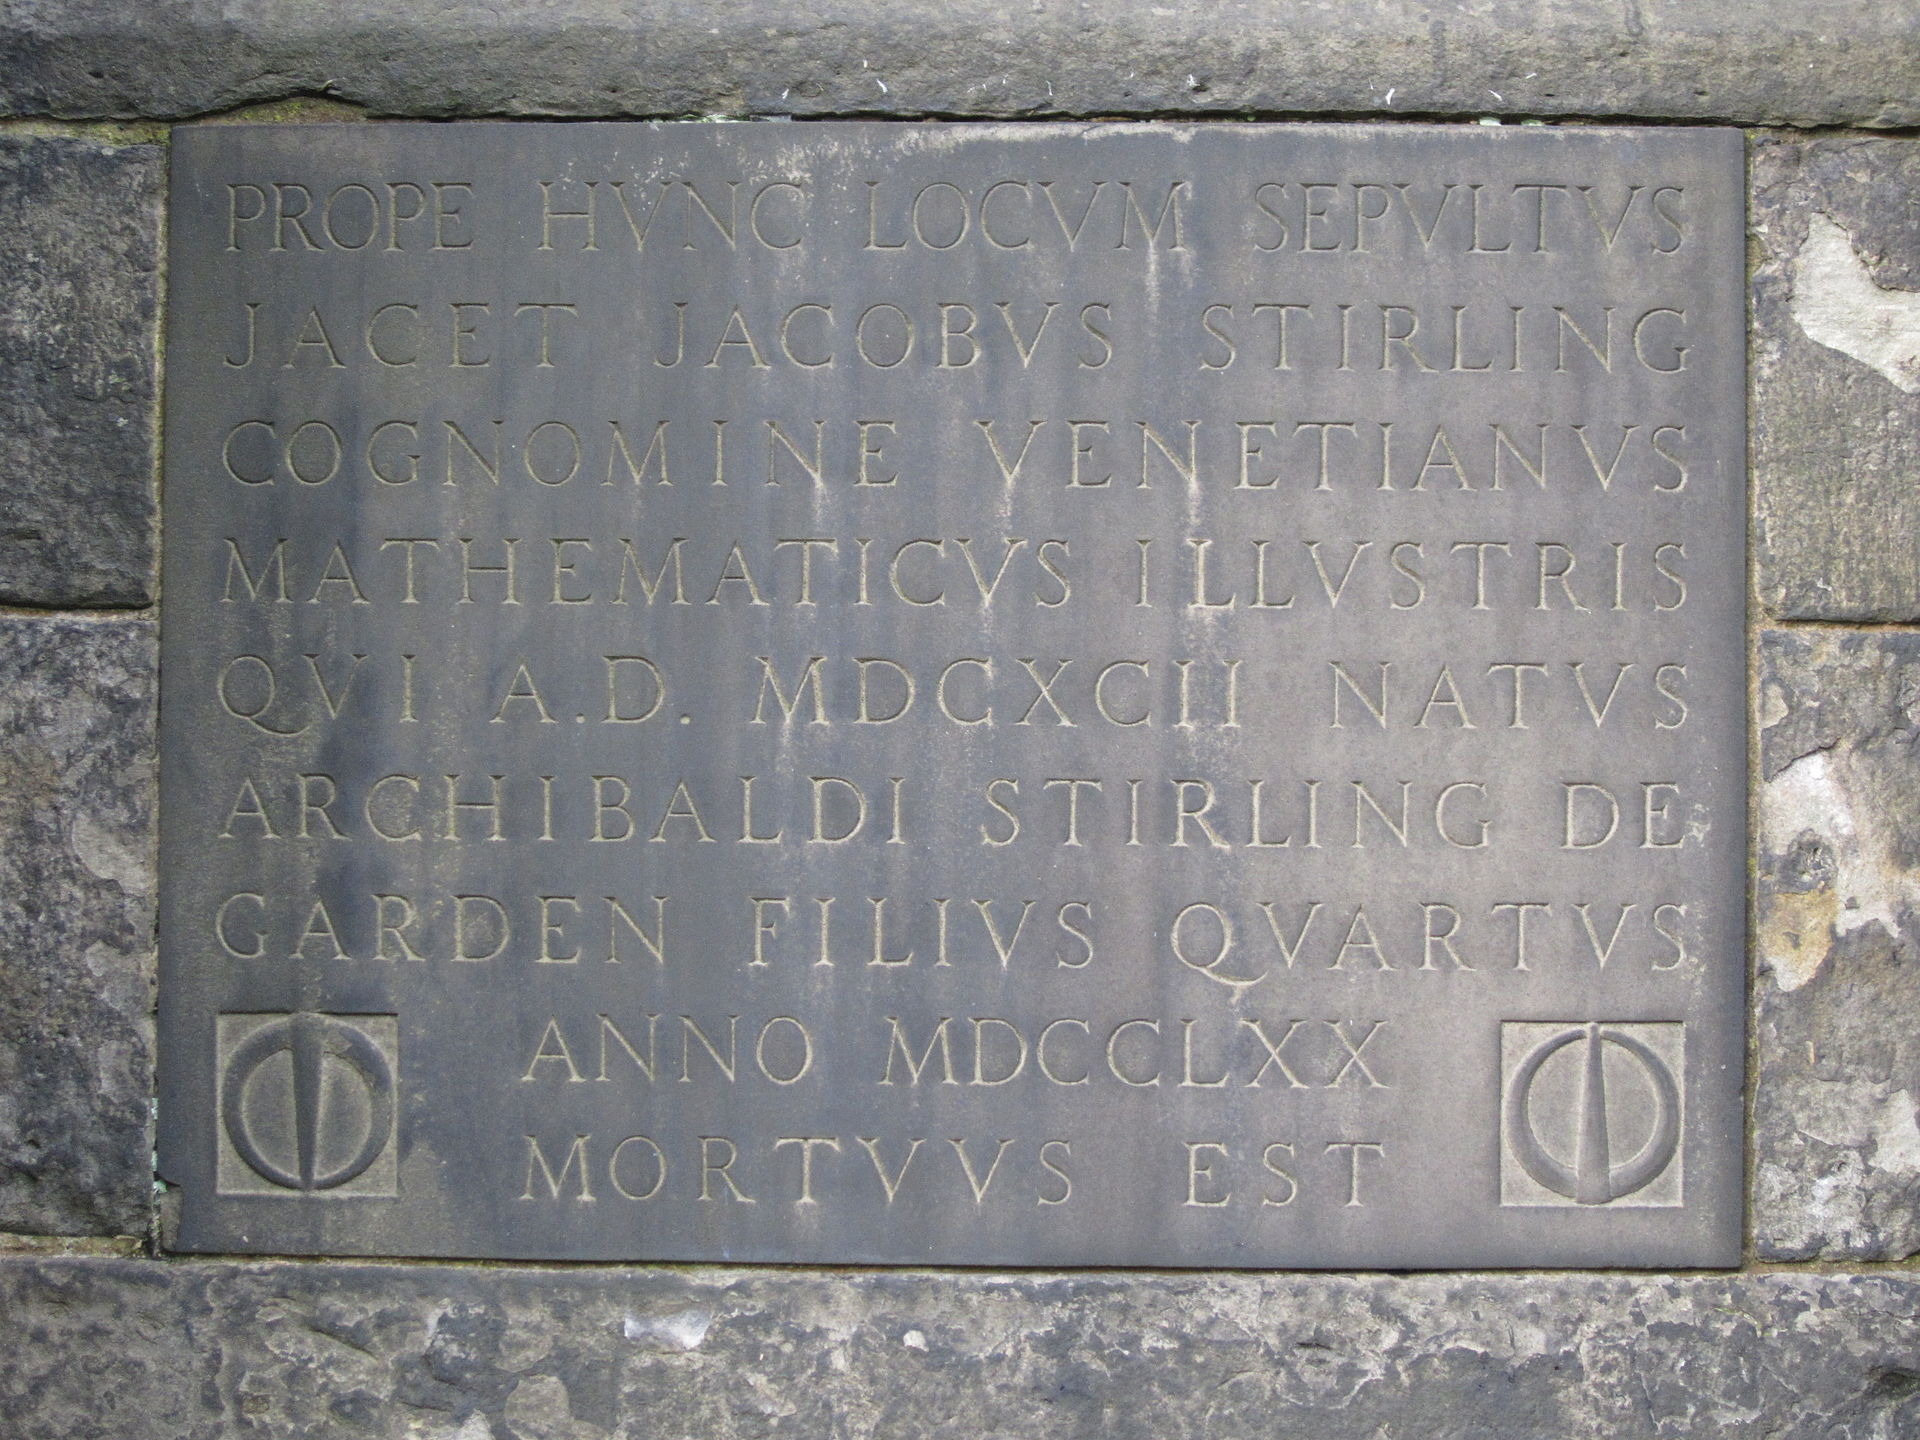
\includegraphics[width=0.4\textwidth]{gamma/stirling_grave.jpg}
\caption{斯特林的墓}
\end{figure}

斯特林的插值研究成果发表于他1730年出版的《Methodus Differentialis》中,由于原书
是拉丁文写成的,有人把他翻译成了英文,并对斯特林的研究成果提供了很多的评论,使
得我们有机会追寻斯特林研究的原始足迹。 有了强大的斯特林公式,可以对$n!$ 进行便
捷的近似计算, 而事实上按照斯特林的插值思路,他已经可以近似计算$n$为任何分数的
时候的阶乘。然而斯特林的思路更多只是停留在数值近似计算上,没有把 $n!$ 到分数的
延拓更细致地追究下去。

% http://math.stackexchange.com/questions/109305/how-much-of-stirling-is-in-stirlings-formula
% knuth Why Pi

\section{三封信---伽玛函数的诞生}

和斯特林处在同一个时代的另外一位数学家几乎在同一个时间点也在考虑 $n!$ 的插值问
题,这个人就是哥德巴赫。哥德巴赫的名字在中国可以说是家喻户晓。由于中国数学家在数论
领域的杰出成就,和素数相关的哥德巴赫猜想作为数学皇冠上的明珠就一直吸引着无数中
国人的目光。 哥德巴赫一生都对数列的插值问题保持浓厚的兴趣,他很早就开始考虑阶乘
的插值问题。不过看起来哥德巴赫的思路不同于斯特林,他并不满足于仅仅做近似的数值
计算,他希望能找到一个通项公式,既可以准确地描述$n!$, 又能够同时推广到分数情形
。不过哥德巴赫无法解决这个问题,幸运的是哥德巴赫交友广泛,和当时许多著名的数学
家都有联系,包括莱布尼茨以及数学史中出了最多位数学家的贝努利家族。1722
年他找尼古拉斯·贝努利请教这个阶乘插值问题,不过没有取得任何进展。即便如此,哥德
巴赫却多年来一直不忘思考这个问题,1729年他又请教尼古拉斯·贝努利的弟弟丹尼尔·贝
努利,而丹尼尔于当年10月给哥德巴赫的一封信中给出了漂亮的解答。

\begin{figure}[htbp]
\centering
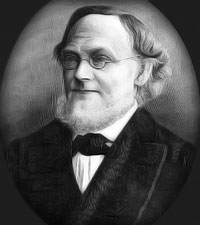
\includegraphics[width=0.25\textwidth]{gamma/goldbach2.jpg}
\quad\quad
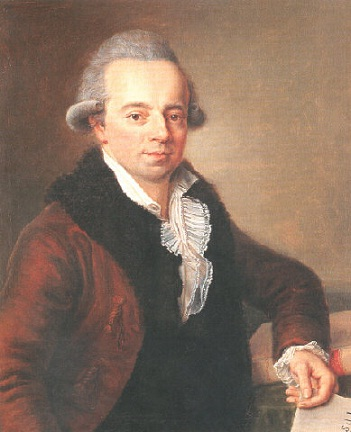
\includegraphics[width=0.25\textwidth]{gamma/Daniel_Bernoulli_by_Grooth.jpg}
\caption{哥德巴赫和丹尼尔·贝努利}
\end{figure}


丹尼尔解决阶乘插值问题的思路非常漂亮:突破有限,取道无穷!他不拘泥于有限的方式
,而是直接跳跃到无穷乘积的形式做插值。丹尼尔发现,如果 $m,n$都是正整数,当 $m
\rightarrow \infty$时,有
$$ \frac{1\cdot 2\cdot 3 \cdots m}{(1+n)(2+n)\cdots (m-1+n)}(m+\frac{n}{2})^{n-1} 
\rightarrow n! .$$
于是利用这个无穷乘积的方式可以把$n!$的定义自然地延拓到实数集。例如,取 $n=2.5$, $m$
足够大,基于上式就可以近似计算出 $2.5!$。我们并不知道丹尼尔是如何想到用无穷乘积
的思路去解决这个问题的,然而他能从有限插值跳跃到无穷,足以显示他优秀的数学才能
。无穷在整个数学发展中发挥着巨大的作用,二十世纪之后的数学笔者不敢妄加评论,然
而如果说“无穷是数学发展的发动机”,在二十世纪之前,这句评论应该不会过分。历次
数学危机是因为无穷而产生,几次数学的重大进展和飞跃也是由于数学家们更加深刻地认
识了无穷。 

接下来伽玛函数的主角欧拉要登场了。欧拉和贝努利家族有着紧密的联系,他是约翰·贝努利
(Johann Bernoulli, 1667-1748)的学生, 这位约翰也就是尼古拉斯和丹尼尔的父亲。我
们应该感谢约翰·贝努利,因为正是他发现并培养了欧拉的数学才能。 在尼古拉斯和丹尼
尔的推荐之下欧拉于1727年在圣彼得堡科学院获得了一个职位。欧拉当时正和丹尼尔·贝努
利一块在圣彼得堡,他也因此得知了阶乘的插值问题。应该是受到丹尼尔·贝努利的思路
的启发,欧拉也采用无穷乘积的方式给出了另外一个$n!$ 的插值公式
\begin{equation}
\label{euler-series}
\Bigl[\Bigl(\frac{2}{1}\Bigr)^n\frac{1}{n+1}\Bigr]
\Bigl[\Bigl(\frac{3}{2}\Bigr)^n\frac{2}{n+2}\Bigr]
\Bigl[\Bigl(\frac{4}{3}\Bigr)^n\frac{3}{n+3}\Bigr] \cdots = n! .
\end{equation}
用极限形式,这个式子以写为
\begin{equation}
\label{euler-series2}
\lim_{m \rightarrow \infty} \frac{1\cdot 2\cdot 3 \cdots m}{(1+n)(2+n)\cdots (m+n)}(m+1)^{n} = n!
\end{equation}
欧拉实际上在他的论文中描述了发现上述式子的思路,我们不在此赘述,不过上式成立却
很容易证明。上式左边可以整理为
\begin{align*}
& \frac{1\cdot 2\cdot 3 \cdots m}{(1+n)(2+n)\cdots (m+n)}(m+1)^{n}  \\
= & \frac{1\cdot 2\cdot 3 \cdots n \cdot (n+1)(n+2) \cdots m}{(1+n)(2+n)\cdots m (m+1)(m+2)\cdots (m+n)}
     (m+1)^{n} \\
= & 1\cdot 2\cdot 3 \cdots n \cdot \frac{(n+1)(n+2) \cdots m}{(1+n)(2+n)\cdots m }
     \cdot \frac{(m+1)^{n}}{(m+1)(m+2)\cdots (m+n)} \\
= & n! \cdot \frac{(m+1)^{n}}{(m+1)(m+2)\cdots (m+n)} \\
= & n! \cdot \prod_{k=1}^{n} \frac{m+1}{m+k}  \\
\rightarrow & n! \qquad (m\rightarrow \infty)
\end{align*}
所以 \eqref{euler-series}、\eqref{euler-series2}式都成立。

而由于\eqref{euler-series} 式对于$n$为分数的情形也适用,所以欧拉实际上也把$n!$
的计算推广到了分数的情形,只是这个计算是用无穷乘积的形式表示的,看起来不够直观
。欧拉给的无穷乘积相比丹尼尔的无穷乘积有什么更出色的地方吗?实际上后人的验证指
出,就收敛到$n!$的速度而言,丹尼尔的无穷乘积比欧拉的要快得多,然而欧拉的无穷乘
积公式却是能够下金蛋的。 欧拉尝试从一些简单的例子开始做计算,看看是否有规律可循
,欧拉极其擅长数学的观察与归纳。当 $n=\frac{1}{2}$ 的时候,带入
\eqref{euler-series} 式,可以得到
\begin{align*}
\Bigl(\frac{1}{2}\Bigr)! 
= & \sqrt{\frac{2}{1}} \cdot \frac{2}{3} \cdot \sqrt{\frac{3}{2}} \cdot \frac{4}{5} 
    \cdot \sqrt{\frac{4}{3}} \cdot \frac{6}{7} \cdot \sqrt{\frac{5}{4}} \cdot \frac{8}{9} 
    \cdot \cdots  \\
= & \sqrt{\frac{4}{2}} \cdot \frac{2}{3} \cdot \sqrt{\frac{6}{4}} \cdot \frac{4}{5}
    \cdot \sqrt{\frac{8}{6}} \cdot \frac{6}{7} \cdot \sqrt{\frac{10}{8}} \cdot \frac{8}{9} 
    \cdot \cdots  \\
= & \sqrt{\frac{4}{3} \cdot \frac{2}{3}} \cdot \sqrt{\frac{6}{5} \cdot \frac{4}{5}}
    \cdot \sqrt{\frac{8}{7} \cdot \frac{6}{7}} \cdot \sqrt{\frac{10}{9} \cdot \frac{8}{9}} 
    \cdot \cdots  \\
= & \sqrt{\frac{2}{3} \cdot \frac{4}{3} \cdot \frac{4}{5} \cdot \frac{6}{5}
    \cdot \frac{6}{7} \cdot \frac{8}{7} \cdot \frac{8}{9} \cdot \frac{10}{9} \cdot \cdots } 
\end{align*}
对比一下根号内的式子和沃利斯公式\eqref{wallis-formula},几乎是一模一样,只是最
前面差了一个因子2。 欧拉自然非常熟悉沃利斯的工作,基于沃利斯公式,欧拉迅速得到了
如下一个令他惊讶的结果
$$ \Bigl(\frac{1}{2}\Bigr)! = \frac{\sqrt{\pi}}{2} .$$

\begin{figure}[htbp]
\centering
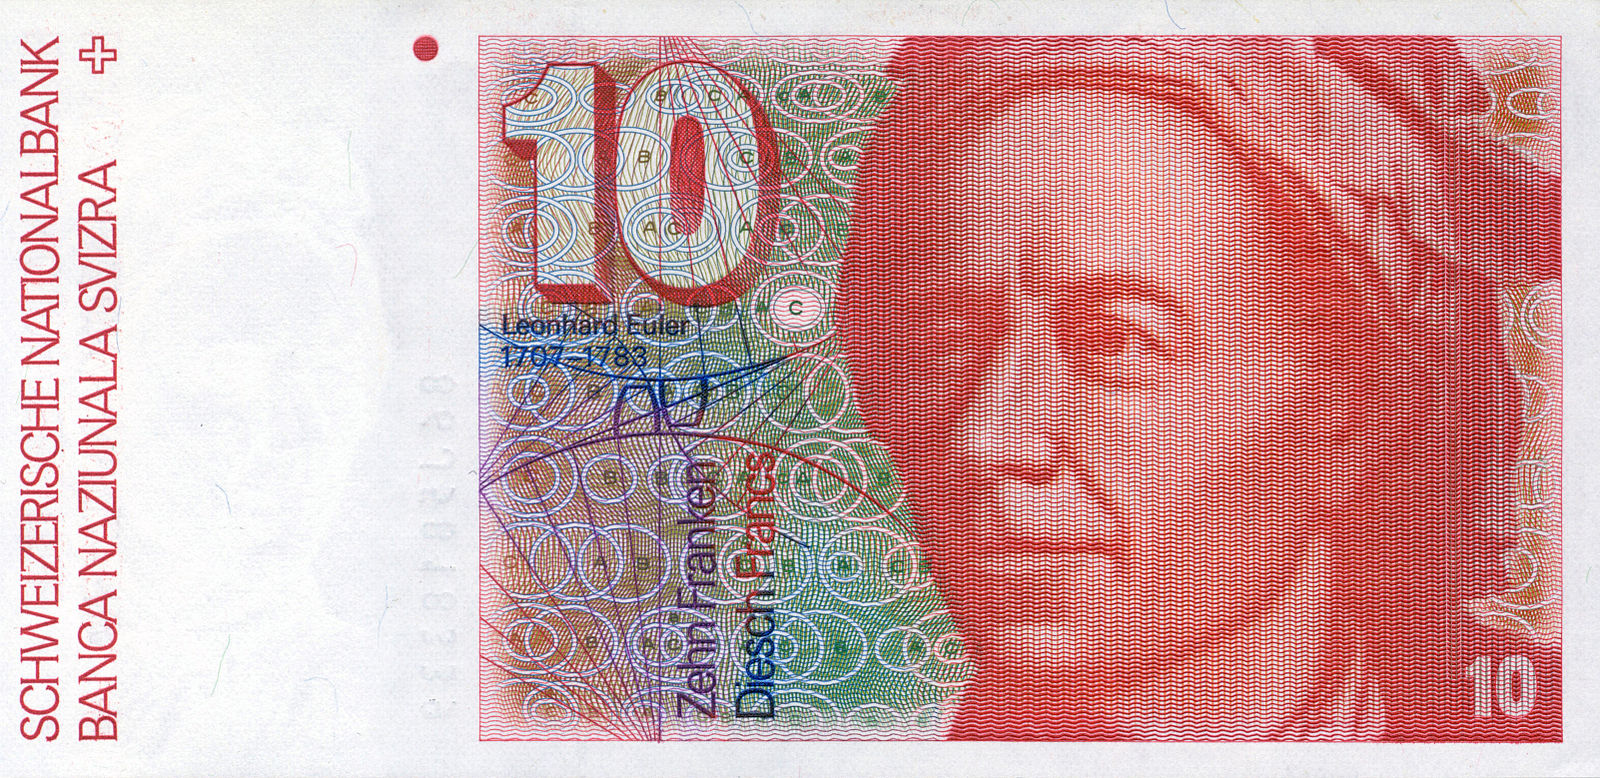
\includegraphics[width=0.8\textwidth]{gamma/euler-swiss-banknote.jpg}
\caption{瑞士法郎上的欧拉}
\end{figure}

欧拉给的无穷乘积满足阶乘的递归式$T(z) = z T(z-1)$, 结合递归式和计算技巧欧拉还计
算了其它几个分数,包括 $\frac{5}{2}, \frac{1}{4}, \frac{3}{4}, \frac{1}{8},
\frac{3}{8} $ 等分数的阶乘。在丹尼尔的鼓励之下,欧拉把自己的插值公式以及一些分
数阶乘的计算结果写信告知了哥德巴赫,这开启了欧拉和哥德巴赫之间一生的通信交流。
两人在接下来的 35 年里连续通信达到196封,这些信函成为了数学家们研究欧拉的重要资
料,而著名的哥德巴赫猜想就是首次出现在哥德巴赫写给欧拉的一封信中,也正是哥德巴
赫激发了欧拉对数论的兴趣。

欧拉是具有超凡的数学直觉的数学家,他看到 $ (\frac{1}{2})!$ 中居然有 $\pi$, 对于
擅长数学分析的数学家而言,有 $\pi$ 的地方必然有和圆相关的积分。同时由于计算$
(\frac{1}{2})!$ 过程中使用到的沃利斯公式,实际上也是计算积分的产物,由此欧拉猜
测 $n!$ 应该可以表达为积分形式,于是欧拉开始努力尝试把 $n!$ 表达为某种积分。虽
然沃利斯的时代微积分的系统理论还没有发明出来,沃利斯使用插值的方式做一些推导计
算,但是沃利斯公式的推导过程本质上就是在处理积分。 如果说沃利斯当年只是无心插
柳,那后继者欧拉是发现了一片绿洲。 受沃利斯工作的启发,欧拉开始考虑如下一般形式
的积分
$$ J(e,n) = \int_0^1 x^e(1-x)^ndx$$
此处 $n$ 为正整数,$e$ 为正实数。利用分部积分法,很容易证明
$$ J(e,n) = \frac{n}{e+1}J(e+1,n-1) $$
重复使用上述迭代公式,最终可以得到
$$ J(e,n) = \frac{1\cdot2\cdots n}{(e+1)(e+2)\cdots(e+n+1)} $$
于是欧拉得到如下一个重要的式子
\begin{equation}
n! = (e+1)(e+2)\cdots(e+n+1)\int_0^1 x^e(1-x)^ndx
\end{equation}
在这个公式里欧拉实际上已经成功地把$n!$ 表示成了积分的形式。然而这里的问题是
$(e+1)(e+2)\cdots(e+n+1)$ 这个表达式限制了 $n$ 只能为整数,无法推广到分数的情形
,欧拉继续研究能否简化这个积分表达式。此处$e$ 是一个任意实数,有没有办法让$e$
从上面的积分式子中消失呢?要让一个量从一个数学等式中消失,数学家们惯用的手法之
一就是让这个量取一个极端的值,譬如无穷。欧拉的老师约翰·贝努利说过“无穷是上帝的
属性”,在通往无穷的路途中,造物主的秘密往往被数学家们窥视。欧拉开始追问:如果
让$e$ 趋向于无穷取值,会发生什么样的情况呢?分析学的大师欧拉开始展现他的计算技
巧,取
$e=\frac{f}{g}$, 稍微整理一下可以得到
$$ \frac{n!}{(f+g)(f+2g)\cdots(f+ng)} = \frac{f+(n+1)g}{g^{n+1}} \int_0^1 x^\frac{f}{g}(1-x)^n dx $$
然后令 $f \rightarrow 1, g \rightarrow 0$,显然上式左边趋于$n!$, 右边会发生什么
情况呢?为了简化计算,令 $x=t^h, h=\frac{g}{f+g}$, 整理之后上式可以变换为
\begin{align}
\frac{n!}{(f+g)(f+2g)\cdots(f+ng)}
& = \frac{f+(n+1)g}{g^{n+1}} \int_0^1 h(1-t^h)^n dt  \notag \\
& = \frac{f+(n+1)g}{(f+g)^{n+1}} \int_0^1 \Bigl(\frac{1-t^h}{h}\Bigr)^n dt 
\label{factorial-integral}
\end{align}
当$f \rightarrow 1, g \rightarrow 0$ 时显然有$h \rightarrow 0$,利用罗必塔法则
,我们可以得到微积分中一个熟知的式子
$$ \lim_{h \rightarrow 0} \frac{1-t^h}{h} = -\log t .$$
于是对 \eqref{factorial-integral} 式两边取极限,奇迹出现了
\begin{equation}
\label{factorial-gamma-1}
n! = \int_0^1 (-\log t)^ndt, 
\end{equation}
原来的积分式中的$e$消失了,欧拉成功地把$n!$表达为了一个非常简洁的积分形式!!!
对上式再做一个变换 $t=e^{-\lambda}$,就可以得到我们常见的伽玛函数形式
\begin{equation}
\label{factorial-gamma-2}
 n! = \int_0^{\infty} \lambda^ne^{-\lambda}d\lambda .
\end{equation}
把\eqref{factorial-gamma-1}和\eqref{factorial-gamma-2} 式从整数$n$ 延拓到任意实
数$x$(包括负数),我们就得到伽玛函数的一般形式
$$ \Gamma(x+1) = \int_0^1 (-\log t)^{x}dt =  \int_0^{\infty} t^{x}e^{-t}dt .$$
1730年 欧拉把他推广得到的$n!$的积分形式再次写信告知了哥德巴赫,由此完美地解决了
困扰哥德巴赫多年的插值问题,同时正式宣告了伽玛函数的诞生,当时欧拉只有23岁。
\begin{figure}[htbp]
\centering
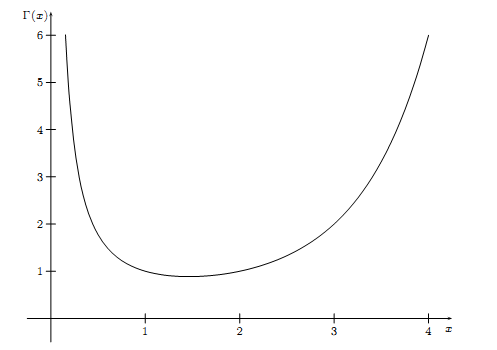
\includegraphics[width=0.6\textwidth]{lda/gamma-func.png}
\caption{$\Gamma(x)$ 在正半轴的图像}
\end{figure}

虽然会有一些争议,有不少数学人把数学家排名中的头两把交椅划给了欧拉和高斯。欧拉
和高斯都是具有超凡直觉的一流数学家,但是欧拉和高斯的风格迥异。高斯是个老狐狸,
数学上非常严谨,发表结果的时候却都把思考的痕迹抹去,只留下漂亮的结果,这招致了
一些数学家对高斯的批评。而欧拉的风格不同,他的做法是把最基本的东西解释得尽量清
楚,讲明引导他得出结论的思路,经常通过经验直觉做大胆的猜测,他的文章中往往留下
了做数学猜想的痕迹。 拉普拉斯曾说过:“读读欧拉 ,他是我们所有人的老师。”高斯的
评价是:“学习欧拉的著作,乃是认识数学的最好工具。”数学家波利亚在他的名著《数
学与猜想》中列举了许多欧拉做数学研究的例子,对欧拉做数学归纳和猜想的方式推崇备
至。

\begin{figure}[htbp]
\centering
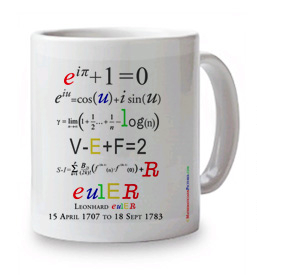
\includegraphics[width=0.4\textwidth]{gamma/euler_cup.jpg}
\caption{欧拉的数学发现}
\end{figure}

欧拉被称为分析学的化身,在分析学中,无出其右者。欧拉的老师约翰·贝努利在给欧拉
的信中这样评价欧拉的工作:“ 我介绍高等分析的时候,它还是个孩子,而你正在将它带
大成人。” 希尔伯特说“分析学是无穷的交响曲”,欧拉显然是无穷分析中最出色的作曲
家。欧拉二百多年前写的教科书《无穷分析引论》至今还在不断地印刷,最近也刚刚出版
了中文翻译版本。布尔巴基学派的灵魂人物韦伊( Andr\'{e} Weil, 1906-1998) 1979 年
在 Rochester大学的一次讲演中说:“今天的学生从欧拉的《无穷分析引论》中所能得到
的益处,是现代的任何一本数学教科书都比不上的。”

许多人把数学比作音乐,把欧拉称作数学界的贝多芬。因为贝多芬在两耳失聪之后继续
谱写了大量著名的交响曲,而欧拉在60岁左右双目失明之后仍然以口述形式完成了几本书
和 400 多篇论文,在数学上变得更加多产。 数学界从1911年开始出版《欧拉全集》,耗
费了一个世纪的时间,已经出版了70余卷, 25000多页, 而这项庞大的出版任务还仍处于
未完成状态。

\section{$ \Gamma(n) = (n-1)!$ 还是  $ \Gamma(n) = n! $ ? }

伽玛函数找到了,我们来看看第二个问题,为何伽玛函数被定义为满足
$\Gamma(n)=(n-1)!$? 这看起来挺别扭的,如果我们稍微修正一下,把伽玛函数定义中的
$t^{x-1}$ 替换为
$t^x$
$$ \Gamma(x) = \int_0^{\infty} t^{x}e^{-t}dt , $$
这不就可以使得 $\Gamma(n)=n!$了嘛。估计数学界每年都有学生问这个问题,然而答案却
一直有一些争议。  

欧拉最早的伽玛函数定义还真是如上所示,选择了$\Gamma(n)=n!$,事实上数学王子高斯
在研究伽玛函数的时候, 一直使用的是如下定义: 
$$ \Pi(x)=\int_{0}^\infty t^x e^{-t}\,dt ,$$ 
然而这个定义在历史上并没有流传开来。 

\begin{figure}[htbp]
\centering
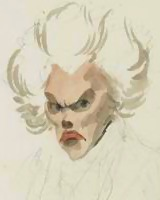
\includegraphics[width=0.25\textwidth]{gamma/Legendre.jpg}
\caption{勒让德肖像水彩画}
\end{figure}

欧拉在伽玛函数的推导中实际上引入了两类积分形式
$$ \int_0^1 t^{x}(1-t)^{y}dt, \quad  \quad \int_0^{\infty} t^{x}e^{-t}dt $$
现在我们分别称为欧拉一类积分和欧拉二类积分。勒让德追随欧拉的脚步,发表了多篇论
文对欧拉积分进行了深入的研究和推广,不过在勒让德的研究中,对积分中的参数做了
$-1$的移位修改,主要定义为
$$ B(x, y) = \int_0^1 t^{x-1}(1-t)^{y-1}dt $$
和
$$ \Gamma(x) = \int_0^{\infty} t^{x-1}e^{-t}dt .$$
$B(x,y)$ 现在称为贝塔积分或者贝塔函数。其中$\Gamma(x)$ 的这个定义选择导致了 $
\Gamma(n) = (n-1)!$ 。实际上伽玛函数中的$\Gamma$符号历史上就是勒让德首次引入的
,而勒让德给出的这个伽玛函数的定义在历史上起了决定作用,该定义被法国的数学家广
泛采纳并在世界范围推广,最终使得这个定义在现代数学中成为了既成事实。

什么原因驱使勒让德偏向选择$\Gamma(n) = (n-1)!$ 的定义呢? 这成为了一个谜,没有
明确地解释。 不过有数学史研究者们对欧拉的研究表明,在$1730\sim1768$ 年之间欧拉
自己在研究一类积分的时候,实际上就已经对积分中的参数做了$-1$的移位修改,从而明
确的引入了贝塔积分,而这个修改显然被勒让德注意到了。 是什么原因使得欧拉和勒让德
在研究他们的积分形式的时候都考虑引入$-1$ 移位修改呢? 有数学家猜测一个可能的原
因是这两位数学家注意到,如果按照现代伽玛函数的定义,那么有
\begin{equation}
\label{beta-gamma-decompose}
 B(x,y) = \frac{\Gamma(x)\Gamma(y)}{\Gamma(x+y)} ,
\end{equation}
$B(x,y)$ 具有非常漂亮的对称形式。可是如果选取高斯给出的 $\Pi(n)=n!$ 的定义,令
$$ E(x, y) = \int_0^1 t^{x}(1-t)^{y}dt $$
则有
$$ E(x,y) = \frac{\Pi(x)\Pi(y)}{\Pi(x+y+1)} ,$$
这个形式显然不如 $B(x,y)$ 具有对称美,而数学家总是很在乎数学公式的美感的。

还有一个类似的解释是从抽象代数的角度提出的,考虑伽玛分布的概率密度函数
$$ f_\alpha(x)=\begin{cases} \dfrac{x^{\alpha-1} e^{-x}}{\Gamma(\alpha)} 
& \text{for }x>0 \\[12pt] 0 & \text{for }x<0 \end{cases} $$
形成的集合 $\{f_\alpha : \alpha > 0\}$, 那么该集合在卷积运算 $*$ 之下构成一
个抽象代数中的半环,即满足
$$ f_\alpha * f_\beta = f_{\alpha+\beta} .$$
而用$\Pi(x)$ 的定义则无法得到类似的结果。 

另外一个更具启发性的解释也是从抽象代数角度描述的。 对伽玛函数
$$ \Gamma(x) = \int_0^{\infty} e^{-t}t^{x-1}dt $$
做一个线性变换 $h: t \rightarrow ct$,可以得到如下函数
\begin{equation}
\label{generalized-gamma}
\frac{\Gamma(x)}{c^x}  = \int_0^{\infty} e^{-ct} t^x \frac{dt}{t} 
\end{equation}
由此 $dt/t = d \log t$ 可以被看成是乘法群 $(0, \infty)$ 上的一个不变测度,在尺
度伸缩变换下满足不变性:
$$ \frac{d(ct)}{ct} = \frac{dt}{t} .$$
而 $e^{-ct}$ 对应于群上的一个加法特征(additive character) $f$, 满足 
$$f(t+s) =f(t) \cdot f(s) ,$$ 
$t^x$ 对应于群上的一个乘法特征(mulpicative character) $g$, 满足
$$g(t \cdot s) = g(t) \cdot g(s) .$$
由于积分表示的是求和, 所以\eqref{generalized-gamma} 式 被看成是乘法群 $(0,
\infty)$ 上加法特征和乘法特征混合乘积的累积求和。有了这个分解,只要在抽象代数的
有限域上定义了$f$ 和$g$ 这两个映射, 实数域上定义的$\frac{\Gamma(x)}{c^x}$ 函数
就可以被推广到有限域上进行定义,只是无限求和的积分号变成了有限求和符号$\Sigma$
。 进一步,借用贝塔函数和伽玛函数满足的关系式\eqref{beta-gamma-decompose},
$B(x,y)$ 也可以完全类似的在有限域中定义出来, 而这种推广也将变得具有简洁的对
称美。当然,这个理由和欧拉、勒让德的选择无关,而是现代数学家们给出的一个额外的
解释。

\section{伽玛函数欣赏}

伽玛函数从它诞生开始就被许多数学家追逐研究,包括高斯、勒让德、魏尔斯特拉斯、柳
维尔等等,数学家们发现了这个函数大量的奇特性质,在解决许多数学问题的时候是一把
利器。伽玛函数作为阶乘的推广,首先它也满足如下的斯特林公式
$$ \Gamma(x) \approx \sqrt{2\pi}e^{-x}x^{x-\frac{1}{2}} .$$
另外, 伽玛函数不仅可以定义在实数集上,基于复变函数的理论还可以延拓到整个复平面
上。所以我们不仅可以计算$ (\frac{1}{2})!, (-7.5)!$,我们甚至可以计算
$(\frac{1}{2} + \frac{1}{3}i)!$,阶乘的概念居然可以推广到虚数,这真是太神奇了! 
\begin{figure}[H]
\centering
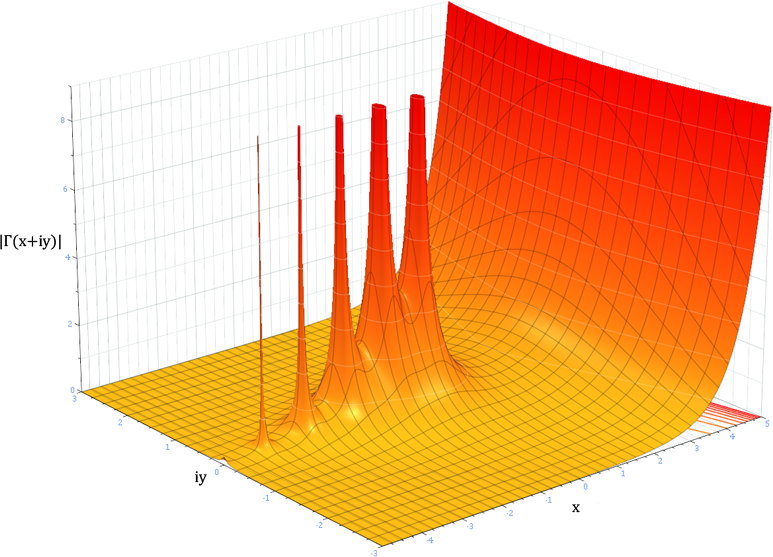
\includegraphics[width=0.5\textwidth]{lda/gamma-complex.png}
\caption{复平面上的伽玛函数}
\end{figure}

欧拉把$n!$ 推广之后得到了伽玛函数,很自然的一个问题是:伽玛函数是$n!$的唯一的
插值推广函数吗? 当然不是,丹尼尔·贝努利最早的无穷乘积推广就已经说明了存在多种
推广延拓的方式。譬如$f(x) = \Gamma(x) \cos (2n\pi)$ 这个函数显然也满足把 $n!$
延拓到实数集。 那伽玛函数在延拓 $n!$ 的时候有什么特殊的地方呢? 从伽玛函数的图
像我们可以看到它是一个凸函数,所以我们很自然地会问伽玛函数是否是唯一的满足凸性
的阶乘函数,可是答案还是否定的。 那伽玛函数为什么鹤立鸡群呢?数学家们发现不仅
$\Gamma(x)$ 是一个凸函数, $\log\Gamma(x)$ 也是一个凸函数,数学上可以证明如下定
理:
\begin{theorem}[Bohr-Mollerup] 如果 $f:(0,\infty)\rightarrow (0,\infty)$,且满足
\begin{enumerate}
\item $f(1) = 1$
\item $f(x+1) = xf(x)$
\item $\log f(x)$ 是凸函数
\end{enumerate}
那么 $f(x) = \Gamma(x)$, 也就是 $\Gamma(x)$是唯一满足以上条件的函数。
\end{theorem}

\begin{figure}[htbp]
\centering
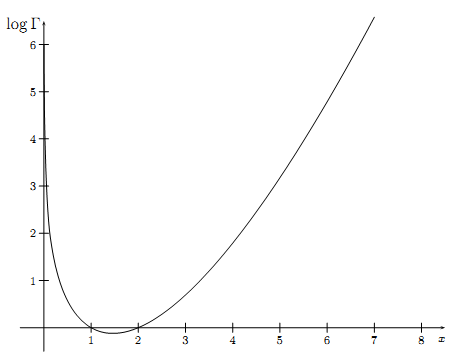
\includegraphics[width=0.45\textwidth]{lda/digamma-func.png}
\caption{$\log \Gamma(x)$ 是一个凸函数}
\end{figure}

伽玛函数有不少等价的表示形式和神奇的结果。高斯给出的伽玛函数的形式是
$$ \Gamma(x) = \lim_{n\rightarrow\infty} \frac{n^x n!}{x(x+1)(x+2)\cdots(x+n)} .$$
欧拉证明了如下一个漂亮的反射公式
$$ \Gamma(x) \Gamma(1-x) = \frac{\pi}{\sin (\pi x)} .$$
魏尔斯特拉斯把高斯的伽玛函数形式做一下变换,就得到如下表达为无穷乘积的结果
$$ {\Gamma(x)} = \frac{1}{xe^{\gamma x}} \prod_{k=1}^\infty
\frac{e^{\frac{x}{k}}} {1+\frac{x}{k}} .$$
此处 $\gamma = 0.5772156649\cdots$ 为欧拉常数。这个结果在复平面上也成立。由于
伽玛函数的这个分解形式的启发,导致魏尔斯特拉斯发现复平面上任意整函数$f(z)$
都可以分解为无穷乘积形式。基于魏尔斯特拉斯的这个无穷乘积形式和欧拉的反射公式,分别
整理简化一下 $\Gamma(1+x)\Gamma(1-x)$,就可以轻松地得到介绍沃利斯公式的时候中提
到的 $\sin x$ 的无穷乘积展开式。 

伽玛函数还有很多妙用,它能扩展一些重要的数学概念,譬如导数。我们可以定义一阶、
二阶等整数阶导数,而数学家们却追问一个奇怪的问题:我们能定义分数阶的导数吗? 这
个问题早年莱布尼茨研究微积分的时候就提出来过,然而没有获得实质性进展。而欧拉
给出了伽玛函数之后,也研究过分数阶导数的问题,并给出了非常具有启发性的想法。我
们观察一下函数$f(x) = x^n$ 的各阶导数

\begin{table}[H]
\centering
\caption{$x^n$ 的各阶导数}
\begin{tabular*}{0.8\textwidth}{@{\extracolsep{\fill}}cl}
\\
$f'(x)$ & $nx^{n-1}$ \\
$f''(x)$ & $n(n-1)x^{n-2}$ \\
$f^{(3)}(x)$ & $n(n-1)(n-2)x^{n-3}$ \\
$\cdots$ &  \\
$f^{(k)}(x)$ & $n(n-1)(n-2)\cdots(n-k+1)x^{n-k} = \frac{n!}{(n-k)!} x^{n-k}$. 
\end{tabular*}
\end{table}

由于$k$阶导数可以用阶乘表达,于是我们用伽玛函数表达为
$$ f(x)^{(k)} = \frac{\Gamma{(n+1)}}{\Gamma{(n-k+1)}} x^{n-k} $$
基于上式,可以把导数的阶从整数延拓到实数集。例如,取$n=1, k=\frac{1}{2}$ 我
们可以计算 $f(x)=x$ 的 $\frac{1}{2}$阶导数为
$$ x^{(\frac{1}{2})} = \frac{\Gamma{(1+1)}}{\Gamma{(1-1/2+1)}} x^{1-1/2} 
= \frac{2\sqrt{x}}{\sqrt{\pi}} .$$
由于一般的可导函数 $f(x)$ 可以通过泰勒级数展开表达为幂级数,于是欧拉很容易地想
到借用 $x^n$ 的分数阶导数,可以尝试定义出任意可导函数的分数阶导数。这种方式确实
能够处理不少函数,不过有点遗憾的是在某些函数上是失效的,所以这种简单的基于泰勒
级数进行扩展的方式并非良好定义的,无法适用于所有函数。欧拉并没有在函数的分数阶导
数的问题上进一步深入,但是他的这个想法非常具有启发性,给后来的数学家提供了重要
的线索,并由此发展了数学分析中的一个研究课题:分数微积分 (Fractional Calculus)
。 在这种微积分中,分数阶的导数是具有意义的,而积分作为导数的逆运算,也可以有
分数阶。 这听起来真是很神奇,而伽玛函数正是实现这种神奇的魔术师。

\begin{figure}[htbp]
\centering
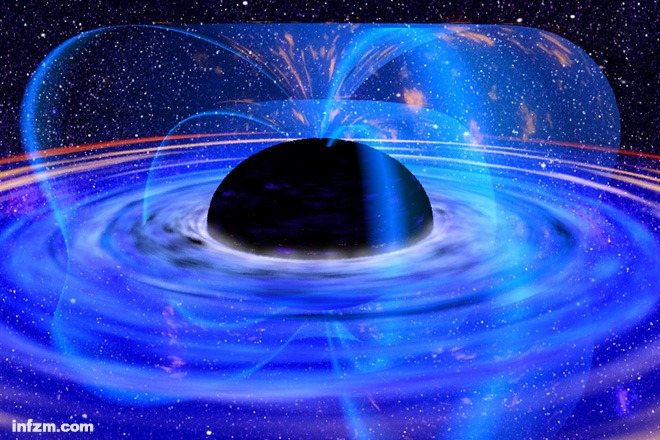
\includegraphics[width=0.4\textwidth]{gamma/n-dim-ball.jpg}
\caption{$n$ 维球的体积}
\end{figure}

伽玛函数还有一个奇妙的运用是求高维空间中球的体积。我们知道 二维球是圆,其面积为
$\pi r^2$;三维球的体积为 $\frac{4}{3} \pi r^3$。那$n$维空间中半径为$r$的球的体
积如何计算呢? 数学上这个体积应该是如下多重积分
$$ \displaystyle V_n(r) = \idotsint\limits_{ \tiny \{(x_1, \cdots, x_n) | \sum x_i^2 < r^2 \} }  1 \quad dx_1dx_2 \cdots dx_n  $$
可以证明
$$ V_n(r) = \frac{\pi^{\frac{n}{2}} r^n}{\Gamma(\frac{n}{2} + 1)} .$$ 
伽玛函数在$n$维球体积公式中扮演了重要角色。 这个公式证明并不难,在 Wikipedia 上可以找到一个很有启发性的证明方法。

下面我们来说一说伽玛函数和数论的关系。 伽玛函数和欧拉常数$\gamma$ 有密切关系,
可以发现
$$ \gamma = -\frac{d\Gamma(x)}{dx}|_{x=1} =
\lim_{n\rightarrow \infty}(1+\frac{1}{2} + \frac{1}{3}+\cdots+\frac{1}{n} - \log n) $$
欧拉常数$\gamma$ 是一个神奇的常数,数学家们至今也没搞清楚它是一个有理数还是一个
无理数。进一步还可以发现伽玛函数和黎曼$\zeta(s)$函数
$$ \zeta(s) = 1+\frac{1}{2^s} + \frac{1}{3^s} + \cdots $$
有密切联系,黎曼发现了如下式子
$$ \zeta(x) \Gamma(x) = \int_0^\infty \frac{u^{x-1}}{e^u - 1} du ,$$
$$ \zeta(x) = \zeta(1-x) \Gamma(1-x) 2^s \pi^{s-1} \sin\left(\frac{\pi x}{2}\right)  .$$
$\zeta$ 函数在解析数论中可是有着举足轻重的地位,因为它涉及了数学中著名的素数分
布定理和黎曼猜想,而以上两个式子在分析黎曼猜想过程中有重要作用。数学家蒙哥马利
有一句名言:“假如你是一个魔鬼,引诱数学家用自己的灵魂来换取一个定理的证明。多
数数学家会想要换取的会是什么定理呢,我想会是黎曼猜想。” 而希尔伯特曾说过,如果
他在沉睡1000年后醒来, 他将问的第一个问题便是:黎曼猜想得到证明了吗?

前面提到了 $\log\Gamma(x)$ 是一个凸函数。对这个函数求导得到的函数
$$ \Psi(x) = \frac{d\log\Gamma(x)}{dx}  $$
被称为 Digamma 函数,可以证明
$$\Psi(x) = -\gamma + (x-1) - \frac{(x-1)(x-2)}{2\cdot 2!} 
+ \frac{(x-1)(x-2)(x-3)}{3\cdot 3!} \cdots $$
这也是一个很重要的函数,具有如下一个漂亮的性质
$$ \Psi(x+1) = \Psi(x) + \frac{1}{x} .$$
基于这个递归性质,把上式在正整数上作递归展开就得到调和级数 $1+\frac{1}{2} +
\frac{1}{3} + \frac{1}{4} + \cdots $,所以$\Psi(x)$ 在调和级数研究中扮演重要角
色。 进一步,函数$\Psi(x)$和欧拉常数$\gamma$ 以及 $\zeta$ 函数都有密切关系,令
$$ \Psi_n(x) = \frac{d^{n+1}\log\Gamma(x)}{dx^{n+1}} ,$$
可以证明
$$\Psi_1(x) = \frac{d^{2}\log\Gamma(x)}{dx^{2}}
= \frac{1}{x^2} + \frac{1}{(x+1)^2} + \frac{1}{(x+2)^2} + \cdots .$$
对于几个具体的数值,有如下漂亮的结果
$$\Psi(1) = -\gamma, \quad \quad \Psi(2) = 1-\gamma $$
$$\Psi_1(1) = \zeta(2) = 1 + \frac{1}{2^2} + \frac{1}{3^2} + \frac{1}{4^2} +  \cdots 
= \frac{\pi^2}{6} $$


\section{随机数学中的伽玛函数}

伽玛函数在概率统计中频繁现身,众多的统计分布,包括常见的统计学三大分布($t$ 分布
,$\chi^2$ 分布,$F$ 分布)、贝塔分布、狄利克雷分布的密度公式中都有伽玛函数的
身影。当然发生最直接联系的概率分布是直接由伽玛函数变换得到的伽玛分布。对伽玛函
数的定义做一个变形,就可以得到如下式子
$$ \int_0^{\infty} \frac{x^{\alpha-1}e^{-x}}{\Gamma(\alpha)}dx = 1 .$$
于是,取积分中的函数作为概率密度,就得到一个形式最简单的伽玛分布的密度函数
$$Gamma(x|\alpha) = \frac{x^{\alpha-1}e^{-x}}{\Gamma(\alpha)} .$$
如果做一个变换 $x=\beta t$, 就得到伽玛分布的更一般的形式
$$Gamma(t|\alpha, \beta) = \frac{\beta^\alpha t^{\alpha-1}e^{-\beta t}}{\Gamma(\alpha)} .$$

\begin{figure}[htbp]
\centering
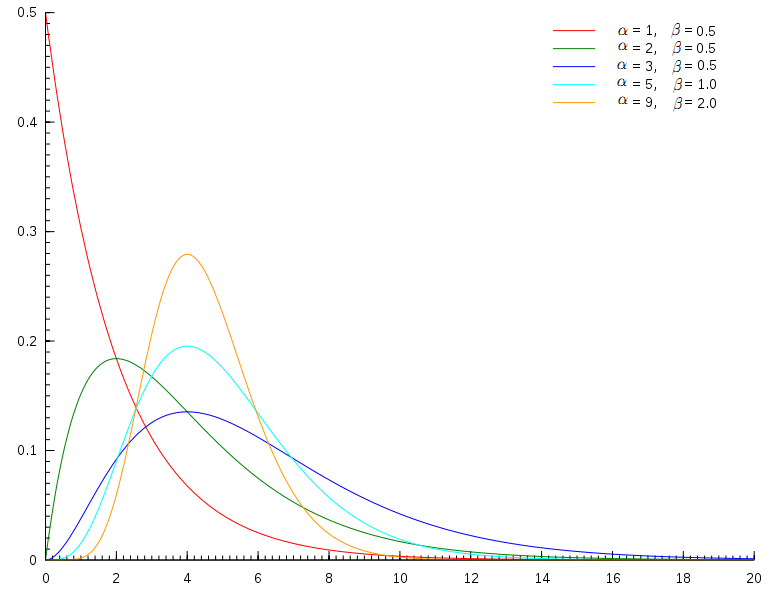
\includegraphics[width=0.6\textwidth]{lda/gamma-distribution.png}
\caption{$Gamma(t|\alpha,\beta)$分布图像}
\end{figure}

伽玛分布在概率统计领域也是一个万人迷,众多统计分布和它有密切关系。指数分布和
$\chi^2$ 分布都是特殊的伽玛分布。另外伽玛分布是一个很强大的先验分布,在贝叶斯统
计分析中被广泛的用作其它分布的先验。如果把统计分布中的共轭关系类比为人类生活中
的情侣关系的话,那指数分布、泊松分布、正态分布、对数正态分布都可以是伽玛分布的
情人。

接下来的内容中我们主要关注$\beta = 1$的简单形式的伽玛分布。伽玛分布首先和泊松分
布发生密切的联系。我们容易发现伽玛分布的概率密度和泊松分布在数学形式上具有高度
的一致性。参数为$\lambda$的泊松分布,概率写为
$$Poisson(X=k|\lambda) = \frac{\lambda^k e^{-\lambda}}{k!} $$
在伽玛分布的密度中取 $\alpha = k+1$ 得到
$$ Gamma(\lambda|\alpha=k+1) 
= \frac{\lambda^ke^{-\lambda}}{\Gamma(k+1)}= \frac{\lambda^k e^{-\lambda}}{k!} $$
所以这两个分布的数学形式具有高度的一致性,只是泊松分布是离散的,伽玛分布是连续
的。这种数学上的一致性是偶然的吗? 事实上,从泊松分布出发,可以利用一个简单的
概率物理模型对伽玛分布的密度函数给出清晰的解释。

泊松分布可以用于描述一段时间内事件发生次数的统计性质,譬如接到的电话的次数。假
设我们关心的不是一段有限的时间,而是 $(0, \infty)$ 整个时间轴上接到电话的统计性
质,应该如何来描述呢?我们可以假设接到的电话满足如下性质
\begin{enumerate}
\item 概率在时间轴是独立均匀分布的,即每个等长的时间区间上是否接到电话是独立的
,并且概率分布一样;每一个长度为h的充分小的时间片上接到一个电话的概率正比于时间
片的长度;
\item 每一个充分小时间片上最多只能接到一个电话;
\item 平均而言,假设每个长度为1的单位时间片上接到电话个数是1。
\end{enumerate}
如果我们考察 $[0, \lambda]$ 这个时间区间,那么平均而言,这个长度为 $\lambda$ 的
时间片上应该接到 $\lambda$ 个电话,把这个时间区间分成 $n$ 个独立的小片,那么每
个时间片上接到一个电话的概率恰好是 $p = \lambda/n$。当$n$ 足够大的时候,每个时
间片上只能是接到一个电话或者没有接到电话,恰好对应于成功概率为$p$ 的一个贝努利
实验,于是$n$ 个时间片对应于$n$ 个独立的贝努利实验,所以 $[0, \lambda]$这个时间
区间上接到的电话总数$X$ 应该符合二项分布
$$p(X=k) = \binom{n}{k} p^k(1-p)^{n-k} .$$
由于 $np= \lambda$, 于是 $n$ 趋向于无穷的时候,电话个数$X$将满足参数为
$\lambda$ 的泊松分布
$$p(X=k) = \frac{\lambda^k e^{-\lambda}}{k!} .$$

熟悉随机过程理论的读者马上会发现以上模型实际上是参数为1 的泊松过程。 我们关心的
问题是:什么时候会接到第${k+1}$ 个电话?或者说接到第$k+1$ 个电话的时间点
$Y_{k+1}$ 会是什么概率分布? 形式化的描述就是如何计算如下的概率?
$$ P(\lambda < Y_{k+1} \le \lambda +  d\lambda) = ? $$
上式表明第$k+1$ 个电话落在长度为 $d\lambda$ 的区间 $(\lambda, \lambda +
d\lambda] $ 内,这个概率事件可以分解为两个独立事件
\begin{enumerate}
\item 区间 $(\lambda, \lambda +  d\lambda] $ 内接到一个电话,这个概率是 $d \lambda$
\item 区间 $[0, \lambda]$ 内接到了前$k$ 个电话,这个概率是 
$$ p(X=k) = \frac{\lambda^k e^{-\lambda}}{k!} .$$
\end{enumerate}
于是所求的概率是以上两个事件概率相乘,即
$$ P(\lambda < Y_{k+1} \le \lambda +  d\lambda) = p(X=k) \cdot d \lambda .$$
由于第$k+1$ 个电话必然出现在时间轴上某处,所以把时间轴所有无穷小区间上的概率累
加起来,正好对应于必然事件的概率1,所以有
$$ \int_0^\infty  p(X=k) \cdot d \lambda  = 1 $$
把$P(X=k)$ 带入上式即可得到 
$$ \int_0^\infty \frac{\lambda^k e^{-\lambda}}{k!}  d \lambda  = 1 $$
$$ k! = \int_0^\infty \lambda^k e^{-\lambda} d \lambda $$
上述两式整好就对应于伽玛分布和伽玛函数。所以$Y_{k+1}$ 恰好符合伽玛分布。 我们其
实从泊松分布出发,完全基于概率物理模型,推导出了伽玛函数,而推导的过程也同时给
伽玛分布的密度函数提供了物理解释。

如果我们把$e^\lambda$的泰勒展开式和伽玛函数对照写成如下形式
\begin{align}
e^\lambda & =  \sum_{k=0}^{\infty} {\lambda^k \over k!}  \\
k! & =  \int_0^{\infty} {\lambda^k \over e^\lambda}\ d\lambda. 
\end{align}
我们发现这两个式子形式上具有对偶关系。由于 $\sum$ 和$\int$ 都表示求和, 几乎可
以认为从第一个式子只是把 $e^\lambda$ 和 $k!$ 交换一下就得到了第二个式子。 这两
个式子之间有更多的内在联系吗?事实上有如下一个奇妙的等式成立
\begin{equation}
\label{gamma-e-taylor}
\frac{1}{k!} \int_0^\lambda \frac{\lambda^k}{e^\lambda} d\lambda 
+ \frac{1}{e^\lambda} \sum_{n=0}^k \frac{\lambda^n}{n!} = 1 
\end{equation}

用上面描述的泊松过程的物理模型,可以很容易的证明这个等式。我们把数轴分成
$(0, \lambda]$ 和 $(\lambda, \infty)$ 这两个区间,考察第$k+1$ 个电话接到时间
$Y_{k+1}$ 分别落在这两个区间的概率,当然有
$$ P(Y_{k+1} \le \lambda) + P(Y_{k+1} > \lambda)  = 1 $$
按照上述的物理模型,显然第$k+1$ 个电话的时间落入$(0, \lambda]$ 的概率为
$$ P(Y_{k+1} \le \lambda) = \int_0^\lambda \frac{\lambda^k e^{-\lambda}}{k!}  d \lambda $$
如果第$k+1$ 个电话的时间点落入 $(\lambda, \infty)$,这个事件等价地可以理解为 $(0,
\lambda]$ 上的电话个数不能超过 $k$ 个,由于$(0, \lambda]$ 这个有限时间区间上的
电话次数符合参数为$\lambda$ 的泊松分布, 所以这个概率为
$$  P(Y_{k+1} > \lambda) = \sum_{n=0}^k \frac{\lambda^n e^{-\lambda} }{n!} $$
所以我们得到
\begin{equation}
\label{poisson-gamma-dual}
\int_0^\lambda \frac{\lambda^k e^{-\lambda}}{k!}d\lambda 
+ \sum_{n=0}^k \frac{\lambda^n e^{-\lambda}}{n!} = 1 
\end{equation}
这个式子俗称泊松-伽玛对偶,简单整理一下就是 \eqref{gamma-e-taylor} 式。

由于泊松分布可以看做是二项分布的极限分布,所以我们也可以从二项分布的角度对伽玛
分布进行解释。由于 
$$ e^{-\lambda} = \lim_{n\rightarrow \infty} (1- \frac{\lambda}{n}) ^n $$
所以伽玛分布的概率密度可以重写为
\begin{align*}
\frac{\lambda^k e^{-\lambda}}{k!} 
& = \lim_{n\rightarrow \infty} \frac{\lambda^k (1-\frac{\lambda}{n}) ^n}{k!}  \\
& = \lim_{n\rightarrow \infty} \frac{ n! n^k (\frac{\lambda}{n})^k (1-\frac{\lambda}{n}) ^n}{k! \cdot n!} \\
& = \lim_{n\rightarrow \infty} \frac{(n+k)!}{k!\cdot n!} (\frac{\lambda}{n})^k (1-\frac{\lambda}{n}) ^n  \\
& = \lim_{n\rightarrow \infty} \binom{n+k}{k} (\frac{\lambda}{n})^k (1-\frac{\lambda}{n}) ^n 
\end{align*}
显然上式具有明确的二项分布的物理含义。事实上,二项分布和贝塔分布之间也存在完全
类似\eqref{poisson-gamma-dual} 的一个等式:
\begin{equation}
\label{binomial-beta-dual}
\frac{n!}{k!(n-k-1)!} \int_0^p t^k(1-t)^{n-k-1} dt + \sum_{v=0}^k \binom{n}{v} p^v(1-p)^{n-v} = 1
\end{equation}
如果我们知道$n\rightarrow\infty$时上式中二项分布的极限是泊松分布,而贝塔分布的
极限是伽玛分布,那么就很容易理解 \eqref{poisson-gamma-dual} 其实可以看做是
\eqref{binomial-beta-dual} 的极限形式。 

\section{结语}

作家海明威说:“冰山运动之雄伟壮观,是因为它只有八分之一在水面上。”阶乘,这么
一个简单的基于整数的数学概念,俨然是一座冰山,我们日常看到的只是它浮在水面上的
一角。而数学家们眼光犀利,看出这座山并非只有整数的一角,他们逐步地深入挖掘探索
,挖出了神奇的伽玛函数,把深藏在冰山下的实数域、复数域、甚至有限域都给挖了出来
。而挖掘出来的伽玛函数真是一个魔术师,它跨越了人们的直觉想象,使得许多数学概念
能够神奇地从整数延拓到分数;而伽玛函数同时又在现代数学的各个分支中表演着自己的
神奇技艺。有许多人认为数学的概念是静态的:这些数学概念产生于历史上某一个时刻,
某一位数学大家之手,之后就几乎一成不变了。对于大多数非数学专业的人而言,这种感
觉貌似很自然,毕竟普通读者所接触的几何、代数、微积分这些数学知识都已经体系成熟
,存在了几百甚至上千年。 然而数学的发展其实是先有探索的阶段,然后才有逻辑与体系
,只是我们的数学课本历来偏重后者而忽视前者。而如果我们对数学知识的探索过程有所
了解的话,会发现这些探索也犹如冰山掩藏在水面之下的部分,甚至比露出的尖角还更具
魅力。 

台湾的数学教授蔡聪明先生在数学的科普传播方面写过大量的文章,他在《数学的发现趣
谈》一书中对于数学的创造、发现与发展有一段精彩的论述:“如果你不知道一个定理(
或公式)是怎样发现的,那么你对它并没有真正的了解,因为真正的了解必须从逻辑因果
掌握到创造的心理因果。一个定理的诞生,基本上跟一粒种子在适当的土壤、风雨、阳光
、气候 ... 之下,发芽成一颗树,再开花结果,并没有两样。”本文尝试尽可能的呈现伽
玛函数这颗数学之树的生长历程,可以说伽玛函数的种子最早是沃利斯播下的,欧拉给予
了最好的施肥、灌溉使得种子发芽,而后来众多数学家们的努力使得这颗嫩芽茁壮成长,
最终几乎成长为一颗参天大树。

伽玛函数这颗大树在现代数学中如此繁茂,笔者知识有限仅能描绘它很有限的一部分。这
个函数在数学上魅力独特,不仅能够被一个理科本科生很好的理解,它本身又足够的深刻
,具有很多漂亮的数学性质,历史上吸引了众多一流的数学家对它进行探索研究。美国数
学家 Philip J.Davis 在1959年在《美国数学月刊》上发表了一篇很有名的介绍伽玛函数
的文章,文中对伽玛函数一些特性发现的历史进行了详细的描述,这篇文章获得了
Chauvenet Prize (美国数学会颁发的数学科普奖)。 他在文中最后总结道:

\begin{quotation}
\noindent
\emph{Each generation has found something of interest to say about the gamma function.
Perhaps the next generation will also.}
\kaishu{(每一代人都发现了一些伽玛函数的有趣性质,也许下一代人也会有所发现。)}
\end{quotation}


\section{推荐阅读}

如果希望了解更多阶乘研究以及伽玛函数相关的历史,推荐阅读如下文献:
\begin{itemize}
\item 蔡聰明, 瓦里斯尋$\pi$ 的發現理路,科学月刊, 27(4) 1996
\item 蔡聰明, 瓦里斯公式及其相關的結果,科学月刊, 27(5), 1996 
\item 蔡聰明, 談 Stirling 公式, 数学传播 , 17(2), 1993
\item Philip J. Davis, Leonhard Euler's Integral: A Historical Profile of the Gamma Function, The American Mathematical Monthly, vol. 66, pp. 849-869, 1959 
\item Jacques Dutka, The Early History of the Factorial Function, Archive for History of Exact Sciences, 43 (3), pp. 225-249, 1991
\item Detlef Gronnau, Why is the gamma function so as it is?, Teaching Mathematics and Computer Science, 2003
\item Emil Artin, The Gamma function(English Traslation),  Holt, Rinehart and Winston, Inc., 1964
\item George E. Andrews et al., Special Functions, Cambridge University Press, 2001
\item Ian Tweddle, James Stirling's Methodus Differentialis: An Annotated Translation of Stirling's Text, Springer, 2003
\end{itemize}
% bibliogrphaphy


% 考虑用到最后的总结中
% 法国伟大的数学家庞加莱(Poincare, 1854-1912)说过:我们用逻辑来证明,但是用直觉
% 来发现。逻辑…是不孕的,除非它跟直觉受精。

